\appendix

\newpage
\section{Example Generations}
\label{app:ex}

Representative continuations seeded with approximately $0.5$ seconds of real
video are shown in Figure~\ref{fig:ex}.

\begin{figure*}[t]
    \centering
    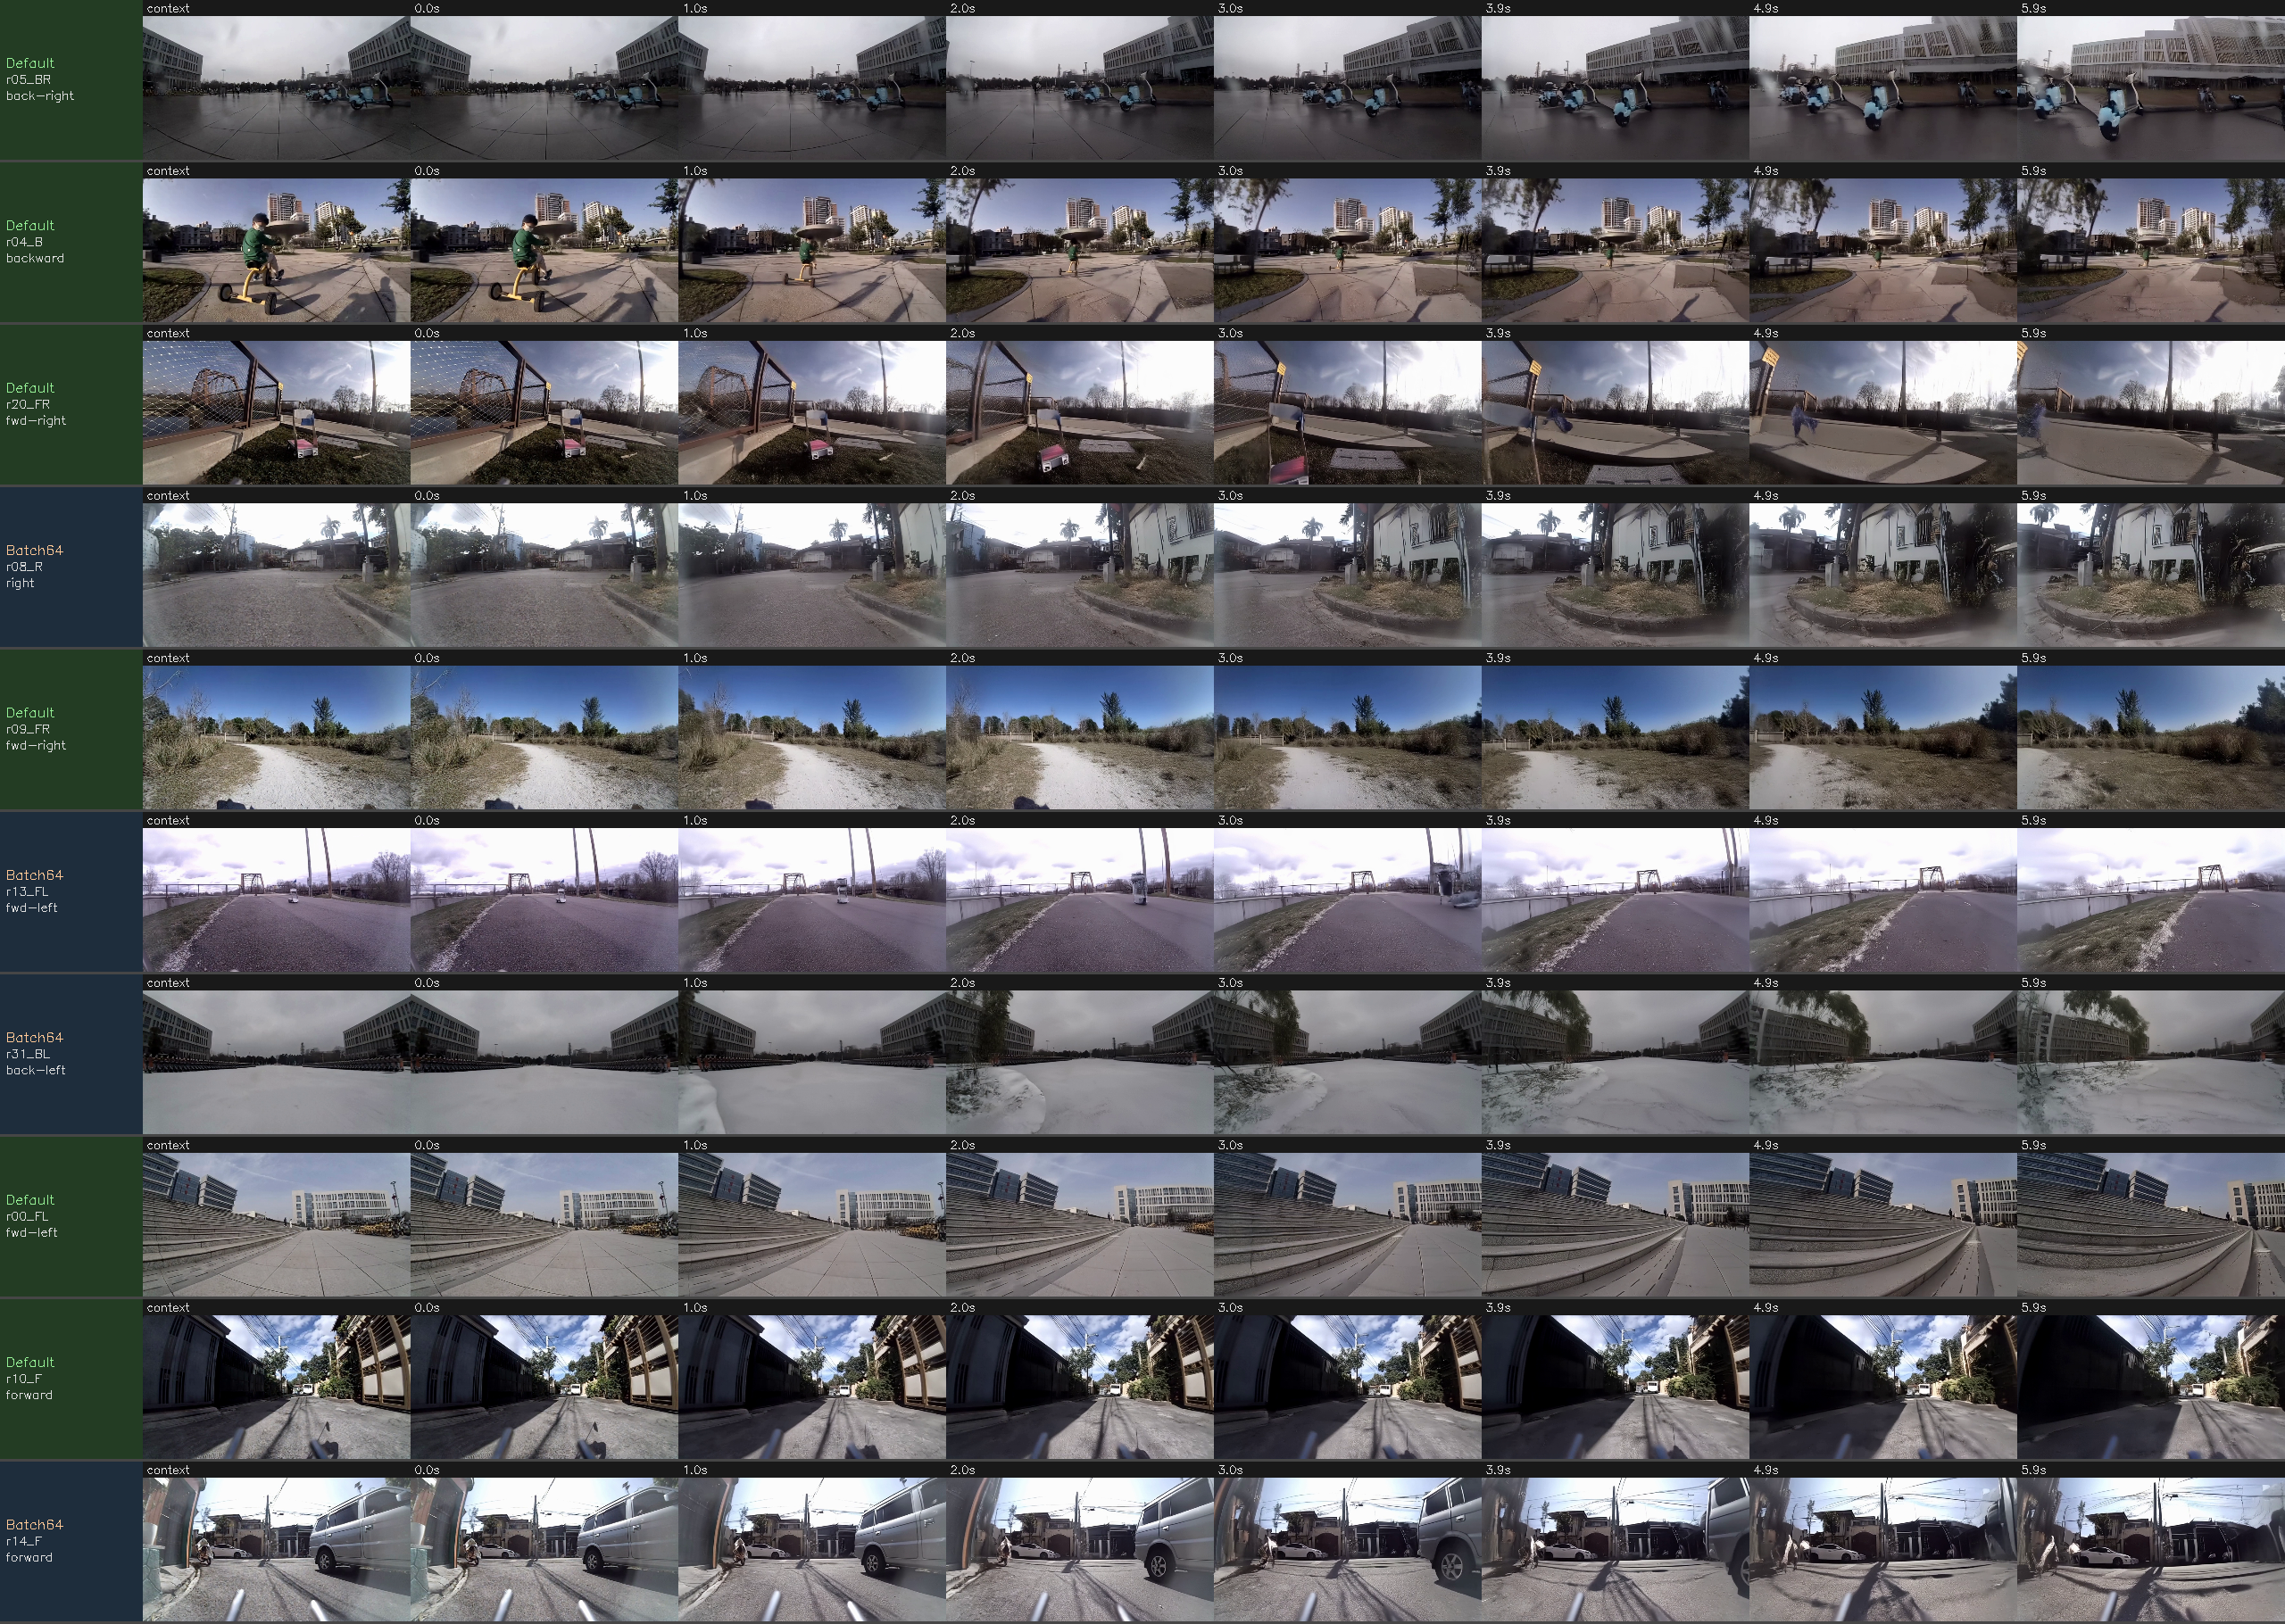
\includegraphics[
        width=0.95\textwidth
    ]{Figures/pca8_showcase_2.png}
    \caption{
        Representative rollouts across environments and cities. The commanded
        action is shown in the leftmost panel of each row.
    }
    \label{fig:ex}
\end{figure*}

\section{Recovered Motion Basis}
\label{app:pca_components}

Figure~\ref{fig:pca_act} visualizes the leading motion directions recovered
by the fixed CoTracker--PCA pipeline. The first component, $g_0$, captures
longitudinal forward--backward motion; $g_1$ captures yaw; and $g_6$ captures
roll-like camera motion. Only $g_0$ and $g_1$ are exposed as control inputs.
The leading eight components are retained as critic targets so that secondary
camera and scene dynamics can regularize generation without enlarging the
two-dimensional control interface.

\begin{figure*}[t]
    \centering
    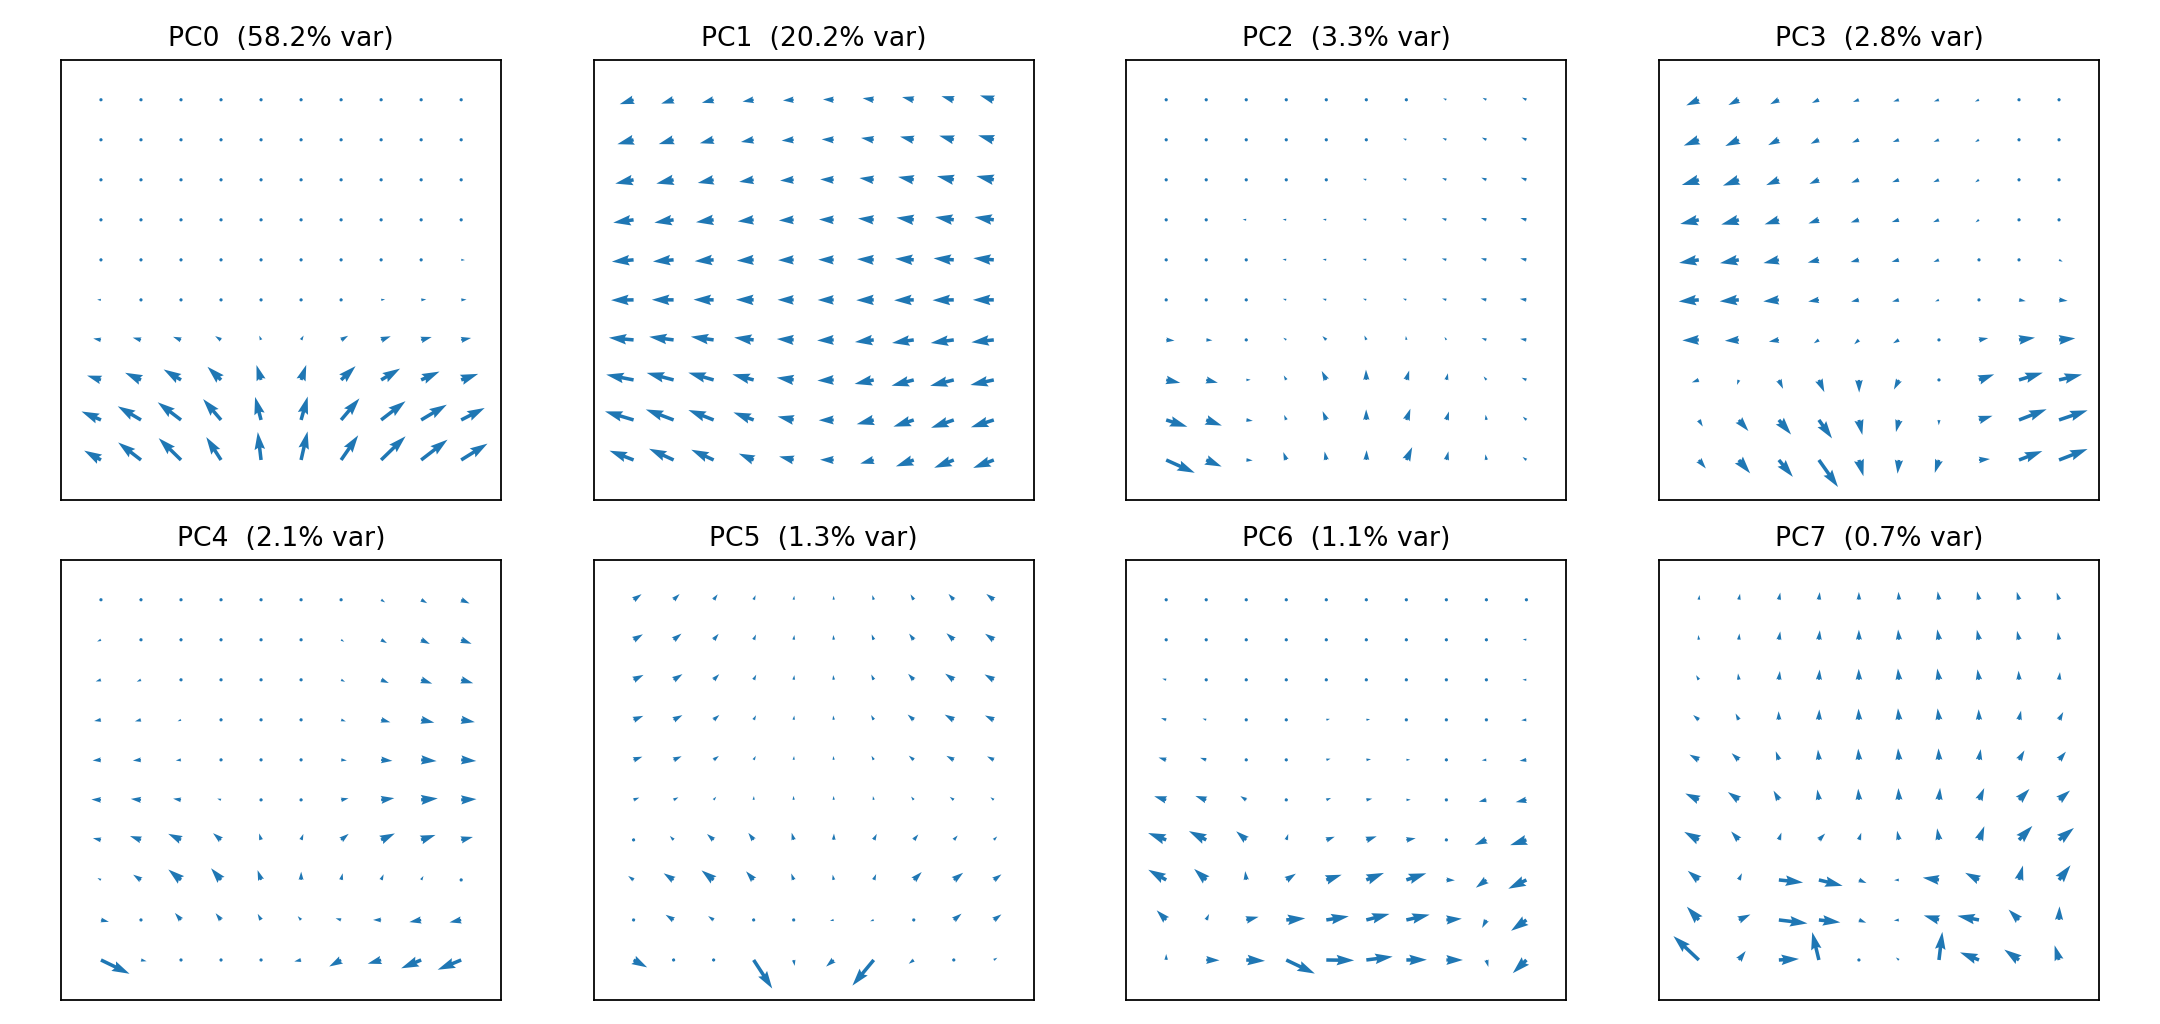
\includegraphics[
        width=0.95\textwidth
    ]{Figures/pca_components_flowfields.png}
    \caption{
        Principal motion components recovered from the fixed
        CoTracker--PCA pipeline. Each panel shows the displacement field
        associated with one PCA coordinate. The exposed control space uses
        $g_0$ for longitudinal motion and $g_1$ for yaw; $g_6$ captures
        roll-like motion. The remaining components describe secondary
        camera and scene dynamics and are used only for critic supervision.
    }
    \label{fig:pca_act}
\end{figure*}

\section{Implementation Details}
\label{app:implementation}

We train and generate autoregressively at the level of temporal latent chunks.
Each training video contains seven chunks and we train using the teacher forcing paradigm \cite{williams1989learning}. We decompose the seven chunk sequence into seven teacher-forced prediction sequences of varying lengths, each targeting one chunk with a different
amount of preceding ground-truth context. Every target therefore has a clean
reference, and a single video provides seven supervised transitions.

At inference, we mirror this factorization by generating one latent chunk at
a time and appending it to the context before predicting the next. This avoids
denoising the complete rollout jointly, keeps the prediction target local, and
allows actions to be changed between successive chunks. When inference is run with 48 diffusion steps like in training, it takes 86s (on a GH200) to generate 7 chunks (or roughly 6 seconds) of content autoregressively, which at 16 FPS gives a generation speed of 1.11 FPS. Since Wan is a flow model, 20 diffusion steps suffice to generate with minimal loss in quality which subsequently increases the generation FPS to 2.72 FPS.  


\section{Cross-Model Evaluation Protocol}
\label{app:evaluation_protocol}

We evaluate directional control using eight compass commands and stationarity
using a separate no-op command. To reduce continuation bias from motion already
present in the conditioning video, we select low-egomotion contexts from held-out
rides.

\subsection{Action-Forcing Benchmark}
\label{app:action_forcing_details}

\paragraph{Low-egomotion context selection.}
The benchmark uses $32$ contexts drawn from distinct held-out FrodoBots rides.
For each candidate window $w$, we compute the mean ego-motion magnitude across
its $N_w$ chunks:
\[
e(w)
=
\frac{1}{N_w}
\sum_{t=1}^{N_w}
\sqrt{
a_{t,\mathrm{throttle}}^2
+
a_{t,\mathrm{yaw}}^2
},
\]
where $a_{t,\mathrm{throttle}}$ and $a_{t,\mathrm{yaw}}$ are the
tanh-squashed PCA action coordinates for chunk $t$.

Let $q_{25}$ denote the $25$th percentile of the ego-motion scores across all
candidate windows. We define the eligibility threshold as
\[
\tau_{\mathrm{stat}}
=
\min(0.12,q_{25}),
\]
and retain candidate windows satisfying
\[
e(w)\leq\tau_{\mathrm{stat}}.
\]
This selects at most the lowest-motion quarter of the candidate population
while also imposing an absolute upper limit of $0.12$ in squashed PCA units.

The selection criterion restricts camera ego-motion rather than all visible
motion. A context may still contain independently moving pedestrians,
vehicles, vegetation, or other scene elements. A separate point-track
scene-activity score is used elsewhere for evaluation but is not part of
this low-egomotion selection criterion.

\paragraph{Commands.}
Each context is continued under the eight constant compass commands
\[
\{
\mathrm{F},\mathrm{FR},\mathrm{R},\mathrm{BR},
\mathrm{B},\mathrm{BL},\mathrm{L},\mathrm{FL}
\},
\]
giving $32\times8=256$ directional rollouts per model. The same source
contexts are used for every model, and each command is held constant throughout
the generated continuation. We additionally generate one no-op continuation
from each context, yielding $32$ stationary rollouts per model. These stationary
rollouts are evaluated separately and are not included in the $256$-rollout
directional fleet.

For our model, actions are ordered as
\[
a=(a_{\mathrm{throttle}},a_{\mathrm{yaw}}).
\]
All commands have Euclidean norm $s=0.5$. The cardinal commands are
\[
\mathrm{F}=(s,0),\qquad
\mathrm{B}=(-s,0),\qquad
\mathrm{R}=(0,s),\qquad
\mathrm{L}=(0,-s),
\]
and the diagonal commands are
\[
\begin{aligned}
\mathrm{FR}&=\frac{s}{\sqrt{2}}(1,1),&
\mathrm{FL}&=\frac{s}{\sqrt{2}}(1,-1),\\
\mathrm{BR}&=\frac{s}{\sqrt{2}}(-1,1),&
\mathrm{BL}&=\frac{s}{\sqrt{2}}(-1,-1).
\end{aligned}
\]
Thus, each active diagonal coordinate has magnitude
$s/\sqrt{2}\approx0.354$. Normalizing the diagonals in this way tests
translation--steering composition without increasing total command magnitude
relative to the cardinal directions.

\paragraph{Context and rollout duration.}
Our model receives one temporal context chunk containing three latent frames,
corresponding to $12$ RGB frames or $0.75$\,s at $16$\,fps. It then generates
eight autoregressive chunks, corresponding to $96$ RGB frames or $6.0$\,s.
The complete context-plus-generation clip therefore contains $108$ RGB frames
and spans $6.75$\,s.

The cross-model benchmark evaluates a common six-second generated horizon.
Each baseline is run through its native autoregressive interface and at its
native output frame rate.

\paragraph{Sampling and reproducibility.}
Our model uses the rectified flow-matching sampler with $48$ denoising steps
per generated chunk, \texttt{timestep\_shift}$=5.0$, and
\texttt{real\_guidance\_scale}$=0.0$, corresponding to no classifier-free
guidance. We evaluate the step-$5{,}000$ checkpoint
\texttt{causal\_lora\_step0005000.pt}. The same sampling configuration is used
for all of our ablations.

Sampling is deterministic. For generated block
$b\in\{0,\ldots,7\}$, the initial noise is drawn using
\[
\mathrm{seed}(b)=1234+b.
\]
The same fixed eight-block noise sequence is reused for every context and
command, holding sampling noise constant across the action-forcing
comparisons.

Each baseline uses its released evaluation checkpoint, sampler, inference-step
count, guidance configuration, and random-seed handling without modification.
The only extensions are the control-interface mappings described in
Section~\ref{app:baseline_controls}.

\paragraph{Evaluation resolution and motion readout.}
Each model is evaluated at its native output resolution; no shared resizing is
applied before the CoTracker--PCA controllability readout. The resolutions are
listed in Table~\ref{tab:action_forcing_resolutions}.

\begin{table}[t]
\centering
{
\small
\begin{tabular}{lc}
\toprule
Model & Output resolution \\
\midrule
Ours                   & $832\times480$  \\
minWM                  & $832\times480$  \\
WorldCam               & $832\times480$  \\
HY-World 1.5 WorldPlay & $832\times480$  \\
Astra                  & $832\times480$  \\
Matrix-Game 2.0        & $640\times352$  \\
Yume-1.5               & $1280\times704$ \\
\bottomrule
\end{tabular}
}
\caption{
    Native output resolutions used by the action-forcing benchmark.
}
\label{tab:action_forcing_resolutions}
\end{table}

The frozen CoTracker--PCA readout is applied independently at each model's
native resolution. Because the conditioning interfaces and native output
resolutions are not metrically matched, raw PCA response magnitudes are not
treated as directly comparable across models. Cross-model analysis instead
emphasizes response sign, requested direction, within-model
forward--backward asymmetry, and translation--steering composition. For the
separate cross-model image-translation analysis, only width-normalized
horizontal and vertical translations are compared.

\paragraph{Failed generations.}
Each context--command rollout is executed independently. If generation fails,
the rollout is skipped entirely: no video or metrics row is written, and the
missing result is not zero-filled or replaced. In practice, after the
control-interface implementations were finalized, all $256$ rollouts
completed successfully for every evaluated model. No benchmark rows were
therefore removed because of generation failure.


\subsection{Baseline Control Interfaces}
\label{app:baseline_controls}

\paragraph{Common protocol.}
Each compass command is translated into the closest operation supported by the
released model and repeated throughout generation. For pose-conditioned
models, the running camera pose is composed with a fixed relative translation
and/or yaw increment. For keyboard--mouse and text-conditioned models, the
corresponding control input or caption is held constant throughout the
rollout. For a given model, all parameters are fixed across scenes and
directions.

The interfaces do not share common physical units. A numerical translation or
rotation used by one model therefore cannot be interpreted as the same
physical command in another model. The benchmark evaluates whether each model
follows the direction and compositional structure of the command expressed
through its own released interface.

In addition to the eight directional commands, each model receives a no-op
command formed as the zero element of its own conditioning interface: a null
pose increment for the pose-conditioned models, an all-zero control stream for
Matrix-Game, and a caption composed from the released still-clauses for Yume.
The specific construction is given for each model below.

\paragraph{minWM}
minWM accepts an autoregressive sequence of relative $\mathrm{SE}(3)$ camera
poses. We use the released trajectory-generator increments of $0.08$
translation and $3^\circ$ yaw per generation step. Forward and backward use
positive and negative longitudinal translation, left and right use signed
yaw, and diagonal commands combine the corresponding translation and yaw
increments. The no-op command uses zero translation and zero yaw, leaving the relative
pose at identity for every generation step.

\paragraph{HY-World 1.5 WorldPlay}
WorldPlay is also driven using relative $\mathrm{SE}(3)$ camera poses and uses
the released trajectory scale of $0.08$ translation and $3^\circ$ yaw per
step. Its pose-string interface cannot express simultaneous translation and
yaw, so diagonal commands are supplied through the released JSON pose
interface. Backward and backward-diagonal commands use negative longitudinal
translation. The no-op command supplies an identity extrinsic for every frame through the
same JSON pose interface.

\paragraph{Astra}
Astra conditions on a per-frame relative camera pose represented by a
flattened $3\times4$ matrix. We follow the scale used in the released
demonstration code, including its translation increment of $0.03$. The release
provides forward and signed-steering primitives. We construct backward motion
by reversing the longitudinal translation and construct backward-diagonal
commands by combining this translation with the released signed-yaw
primitive. The no-op command holds the identity relative pose $\mathbf{I}_{3\times4}$ for
every frame. This matches the release's own convention: its trajectory
generator already assigns identity poses to the conditioning frames, annotated
as zero-motion camera pose, and our no-op extends that convention across the
generated span rather than switching to a translation increment at the
hand-off.

\paragraph{WorldCam}
WorldCam is conditioned on per-pixel-frame camera-to-world trajectories in
OpenCV convention. Its pose scale is inherited from its training trajectories
and is not metric. Because the release does not include an eight-direction
trajectory generator, we construct one through the released pose interface.

The conditioning span uses identity poses. During generation, the running pose
is composed multiplicatively as
\[
C_{t+1}=C_tD,
\]
where $D$ contains a longitudinal translation of
\[
\Delta z=\pm0.02
\]
camera-to-world units per pixel frame and/or a yaw rotation of
$\pm1.5^\circ$ about the $y$-axis. Positive and negative translations are used
for the forward and backward command families, respectively. Positive yaw is
used for right-family commands and negative yaw for left-family commands.
Diagonal commands combine the corresponding translation and yaw within the
same increment.

The released runner performs $50$ autoregressive steps and produces $200$
generated frames. We use the fixed intrinsics
\[
f_x=f_y=723,\qquad c_x=960,\qquad c_y=540.
\]
The translation unit is arbitrary because WorldCam's pose scale derives from
its training trajectories. The translation and yaw increments were fixed
during interface calibration before the action-forcing benchmark and were
then applied unchanged across every scene and direction. The no-op command sets $D=I$, that is $\Delta z=0$ with zero yaw, so the
running pose $C_{t+1}=C_tD$ remains at the identity of the conditioning span
throughout generation.

\paragraph{Matrix-Game 2.0}
Matrix-Game accepts a six-dimensional binary keyboard stream and a
two-dimensional mouse stream, both held constant throughout generation. We
use its released benchmark mouse-yaw magnitude of $0.1$ per pixel frame. The
eight command mappings are given in
Table~\ref{tab:matrix_game_commands}.

\begin{table}[t]
\centering
{
\small
\begin{tabular}{ccc}
\toprule
Command & Keyboard input & Mouse yaw \\
\midrule
$\mathrm{F}$  & \texttt{forward}=1  & $0$ \\
$\mathrm{B}$  & \texttt{backward}=1 & $0$ \\
$\mathrm{R}$  & none                & $+0.1$ \\
$\mathrm{L}$  & none                & $-0.1$ \\
$\mathrm{FR}$ & \texttt{forward}=1  & $+0.1$ \\
$\mathrm{FL}$ & \texttt{forward}=1  & $-0.1$ \\
$\mathrm{BR}$ & \texttt{backward}=1 & $+0.1$ \\
$\mathrm{BL}$ & \texttt{backward}=1 & $-0.1$ \\
$\varnothing$ & none                & $0$ \\
\bottomrule
\end{tabular}
}
\caption{
    Matrix-Game 2.0 controls used for the eight-direction benchmark.
}
\label{tab:matrix_game_commands}
\end{table}

Keyboard controls are binary, whereas mouse yaw has a continuous magnitude.
Backward input is supported by the released interface but is not exercised in
the model's released benchmark protocol.

\paragraph{Yume-1.5.}
Yume is controlled through natural-language captions drawn from its supported
training vocabulary. Each command uses the common prefix
\begin{quote}
\small
\emph{This video depicts a city walk scene with a first-person view (FPV).}
\end{quote}
followed by the corresponding person and camera clauses in
Table~\ref{tab:yume_commands}. The complete caption is repeated throughout
the rollout. Yume exposes directional commands but no numerical command
magnitude and therefore cannot be evaluated using a continuous dose sweep.

\begin{table}[t]
\centering
{
\small
\begin{tabular}{lll}
\toprule
Command & Person clause & Camera clause \\
\midrule
F  & moves forward (W)              & remains still \\
B  & moves backward (S)             & remains still \\
L  & stands still                   & turns left \\
R  & stands still                   & turns right \\
FL & moves forward and left (W+A)   & turns left \\
FR & moves forward and right (W+D)  & turns right \\
BL & moves backward and left (S+A)  & turns left \\
BR & moves backward and right (S+D) & turns right \\
$\varnothing$ & stands still ($\cdot$) & remains still ($\cdot$) \\
\bottomrule
\end{tabular}
}
\caption{
    Yume-1.5 caption clauses used for the eight-direction benchmark.
}
\label{tab:yume_commands}
\end{table}

\paragraph{Text-conditioning neutrality.}
Several baselines accept a text prompt alongside their action interface. Under
a directional command, motion-referring language in that prompt is harmless;
under a no-op it contradicts the commanded behaviour. Three of the prompts we
used for the directional benchmark contain such language: Astra's scene prompt
ends with ``\emph{The camera moves smoothly through the scene}''; Yume's
common prefix describes a ``\emph{city walk}'' scene; and WorldCam inherits
its base model's default negative prompt, which lists three terms meaning
\emph{static}, \emph{motionless}, and \emph{a still, unmoving picture} among
the artefacts to be avoided, thereby penalising the behaviour under test.

For the stationary evaluation we therefore repeat these rollouts with the
motion-referring language removed and all other settings unchanged.
Neutralisation reduces camera drift substantially for Yume and Astra, leaves
minWM and WorldPlay essentially unchanged, and increases drift for WorldCam.
We use the neutral prompts for Yume and Astra and retain the released defaults
elsewhere, following the rule ``use the released default unless it explicitly
contradicts the command''. The stationary results in
Appendix~\ref{app:stationary_results} use these settings.

\paragraph{Authored interface extensions.}
Our additions operate only through the models' released conditioning
interfaces. We construct backward and backward-diagonal pose sequences for
Astra, backward--yaw combinations for Matrix-Game diagonals, an
eight-direction trajectory generator for WorldCam, and simultaneous
translation--yaw commands through WorldPlay's JSON interface. For the
stationary evaluation we further supply each model with a no-op command
through its native interface: identity pose sequences for the four
camera-conditioned models (minWM, WorldPlay, Astra, WorldCam), an all-zero
keyboard and mouse-control stream for Matrix-Game, and the composed
still-clause caption for Yume. In each case the no-op is the zero element of
the model's own conditioning representation, and for the pose-conditioned
models it coincides with the identity convention those releases already apply
to their conditioning spans.

These inputs are representable by the released conditioning tensors but are
not part of the models' published benchmark protocols, which expose no named
or evaluated no-op command; we therefore report the resulting rollouts as each
model's response to an authored zero-input extension. No model architecture,
learned weight, or conditioning representation is modified.

PCA centres the tracked-motion vectors before projection, so the mean raw PCA
score is zero by construction. However, the numerical score origin corresponds
to the training-set mean tracked-motion field rather than to zero displacement.
We therefore obtain our stationary command by passing an all-zero displacement
field through the same action encoder, giving the calibrated value
$a_{\mathrm{null}}=(-0.0234,-0.0013)$ defined in
Eq.~\eqref{eq:null_action}. This correction cancels the mildly forward/right
mean motion and is used only for the no-op evaluation; all training actions and
all active commands retain their original encoded values. No analogous
calibration is applied to the baselines, whose stationary inputs are the
untuned zero or identity elements of their released interfaces.

\subsection{Response-Curve Protocol}
\label{app:response_details}

\paragraph{Ablation curves.}
The reverse-throttle and steering branches are measured using held-out ride
windows whose recorded commands are replaced by their rotated
counterfactuals. We use evaluations from the final $1{,}000$ training steps,
restrict the window offset to at most $81$, and measure only settled chunks by
discarding the first two generated chunks of each rollout. This is because there is a finite acceleration in the data and rapid direction changes induce a penalty from this acceleration. We find this in a lot of the other baseline models too, so all models use this protocol.

For each action axis, requested values are divided into $13$ linearly spaced
bins spanning the $2$nd to the $98$th percentile of the requested-command
distribution. A bin is plotted only when it contains at least $12$ samples.
Each plotted point is the mean realized CoTracker--PCA response within that
bin. Shaded regions show one standard error of the mean:
\[
\mathrm{SEM}
=
\frac{\operatorname{std}(x)}{\sqrt{n}}.
\]

Genuine reverse travel is too rare to produce a sufficiently populated
rotated forward branch. We therefore measure forward response using
held-out no-op contexts and the fixed positive throttle strengths
\[
\{0.1,0.2,\ldots,0.8\}.
\]
Settled response is again measured after discarding the first two generated
chunks. When more than $132$ samples are available at a command strength, we
subsample $132$ examples using a fixed random seed of $0$. This cap matches
the size of the largest FLIP bin.

The forward and reverse branches therefore probe the same throttle coordinate
but do not use identical starting-context distributions. They are used to
evaluate response sign, smoothness, saturation, and approximate gain rather
than as a paired forward--backward comparison. Dashed plot boundaries mark
the approximate support of the training actions, extending to approximately
$+0.5$ for forward throttle and $-0.3$ for reverse throttle.

\paragraph{Cross-model curves.}
Cross-model response curves use the same $32$ held-out contexts as the
eight-direction action-forcing benchmark. The compass commands produce the
five signed per-axis protocol levels
\[
\left\{
-0.5,\,
-\frac{0.5}{\sqrt{2}},\,
0,\,
\frac{0.5}{\sqrt{2}},\,
0.5
\right\}
\approx
\{-0.5,-0.354,0,0.354,0.5\}.
\]
For each level, the plotted point is the mean response over the $32$ scenes
and the shaded region shows $\pm1$ SEM.

Each baseline receives the corresponding fixed-strength command through its
native interface. The horizontal coordinate represents the signed protocol
level rather than a common physical control magnitude. The curves are
therefore interpreted through response sign and within-model
forward--backward asymmetry rather than absolute cross-model gain. The dotted
diagonal denotes unit gain.

\section{Extended Controllability Results}
\label{app:extended_control}

This section expands the controllability analysis from the main paper. We
first study how the conditioning pathway, batch size, and dimensionality of
critic supervision affect the acquisition of command control. We then report
the settled directional responses of the ablation variants, followed by
additional cross-model analyses of throttle, steering, and the roll-like
motion coupled to yaw.

\subsection{Conditioning-Pathway Ablation}
\label{app:conditioning_ablation}

Figure~\ref{fig:abl_injection} isolates the effect of the action-conditioning
pathway. Injecting actions through both AdaLN and action tokens produces the
fastest convergence and strongest counterfactual response. AdaLN alone still
establishes control, but converges more slowly and reaches a weaker response.
Action tokens alone appear competitive under GT evaluation but fail under
FLIP, showing that continuation of the source motion can be mistaken for
command following.

\begin{figure*}[t]
    \centering
    
\includegraphics[
        width=0.82\textwidth
    ]{Figures/following_FAMILY_injection_by_REALdir.png}
    \caption{
        Conditioning-pathway ablation under counterfactual FLIP evaluation,
        grouped by source-ride motion direction. Dual injection through AdaLN
        and action tokens converges fastest and reaches the strongest response.
        AdaLN-only conditioning learns control more slowly, while tokens-only
        conditioning remains anti-aligned on throttle and unstable on steering.
        Panels and smoothing follow Fig.~\ref{fig:following_dir}.
    }
    \label{fig:abl_injection}
\end{figure*}


\subsection{Training-Time Command Following}
\label{app:extended_control_following}

\paragraph{Default model.}
Figure~\ref{fig:following_8pca} extends the main-paper training analysis to all
eight source-motion groups for the default pca8 model with global batch size
$32$. GT agreement rises early because the pretrained model can continue the
motion already present in the context. FLIP agreement instead measures whether
the supplied action changes that continuation. Steering is acquired first,
while backward and backward-diagonal control emerge later.

\begin{figure*}[t]
    \centering
    
\includegraphics[
        width=0.82\textwidth
    ]{Figures/following_8node8pca_by_REALdir.png}
    \caption{
        Training-time command following for the default model across all eight
        source-motion groups. Blue uses the recorded command (GT), while red applies
        the sign-flipped counterfactual (FLIP) to the same context. Positive FLIP
        agreement indicates genuine command response. Panel titles denote the
        source-context motion, and curves use a $9$-point
        ($\approx450$-step) centred rolling mean.
    }
    \label{fig:following_8pca}
\end{figure*}

\paragraph{Tokens-only conditioning.}
Figure~\ref{fig:noadaln_gt_flip} illustrates why GT agreement is insufficient
on its own. The no-AdaLN, tokens-only variant obtains high GT agreement in
several common source-motion contexts, but its FLIP response remains negative
or unstructured. It therefore continues motion inherited from the context
without acquiring reliable command control.

\begin{figure*}[t]
    \centering
    
\includegraphics[
        width=0.82\textwidth
    ]{Figures/following_noadaln_by_REALdir.png}
    \caption{
        GT and FLIP agreement for the no-AdaLN, tokens-only variant. High GT
        agreement but negative or unstructured FLIP response shows that the model
        continues source motion without acquiring reliable command control. Panel
        titles denote source-context motion.
    }
    \label{fig:noadaln_gt_flip}
\end{figure*}

\paragraph{Larger-batch model.}
Figure~\ref{fig:following_16pca} shows the corresponding training curves for
the Batch64 model. GT agreement again rises rapidly, but FLIP agreement also
becomes consistently positive across all eight directions. Relative to the
default batch size, the larger batch produces smoother training dynamics and
a stronger response in the harder throttle directions.

\begin{figure*}[t]
    \centering
    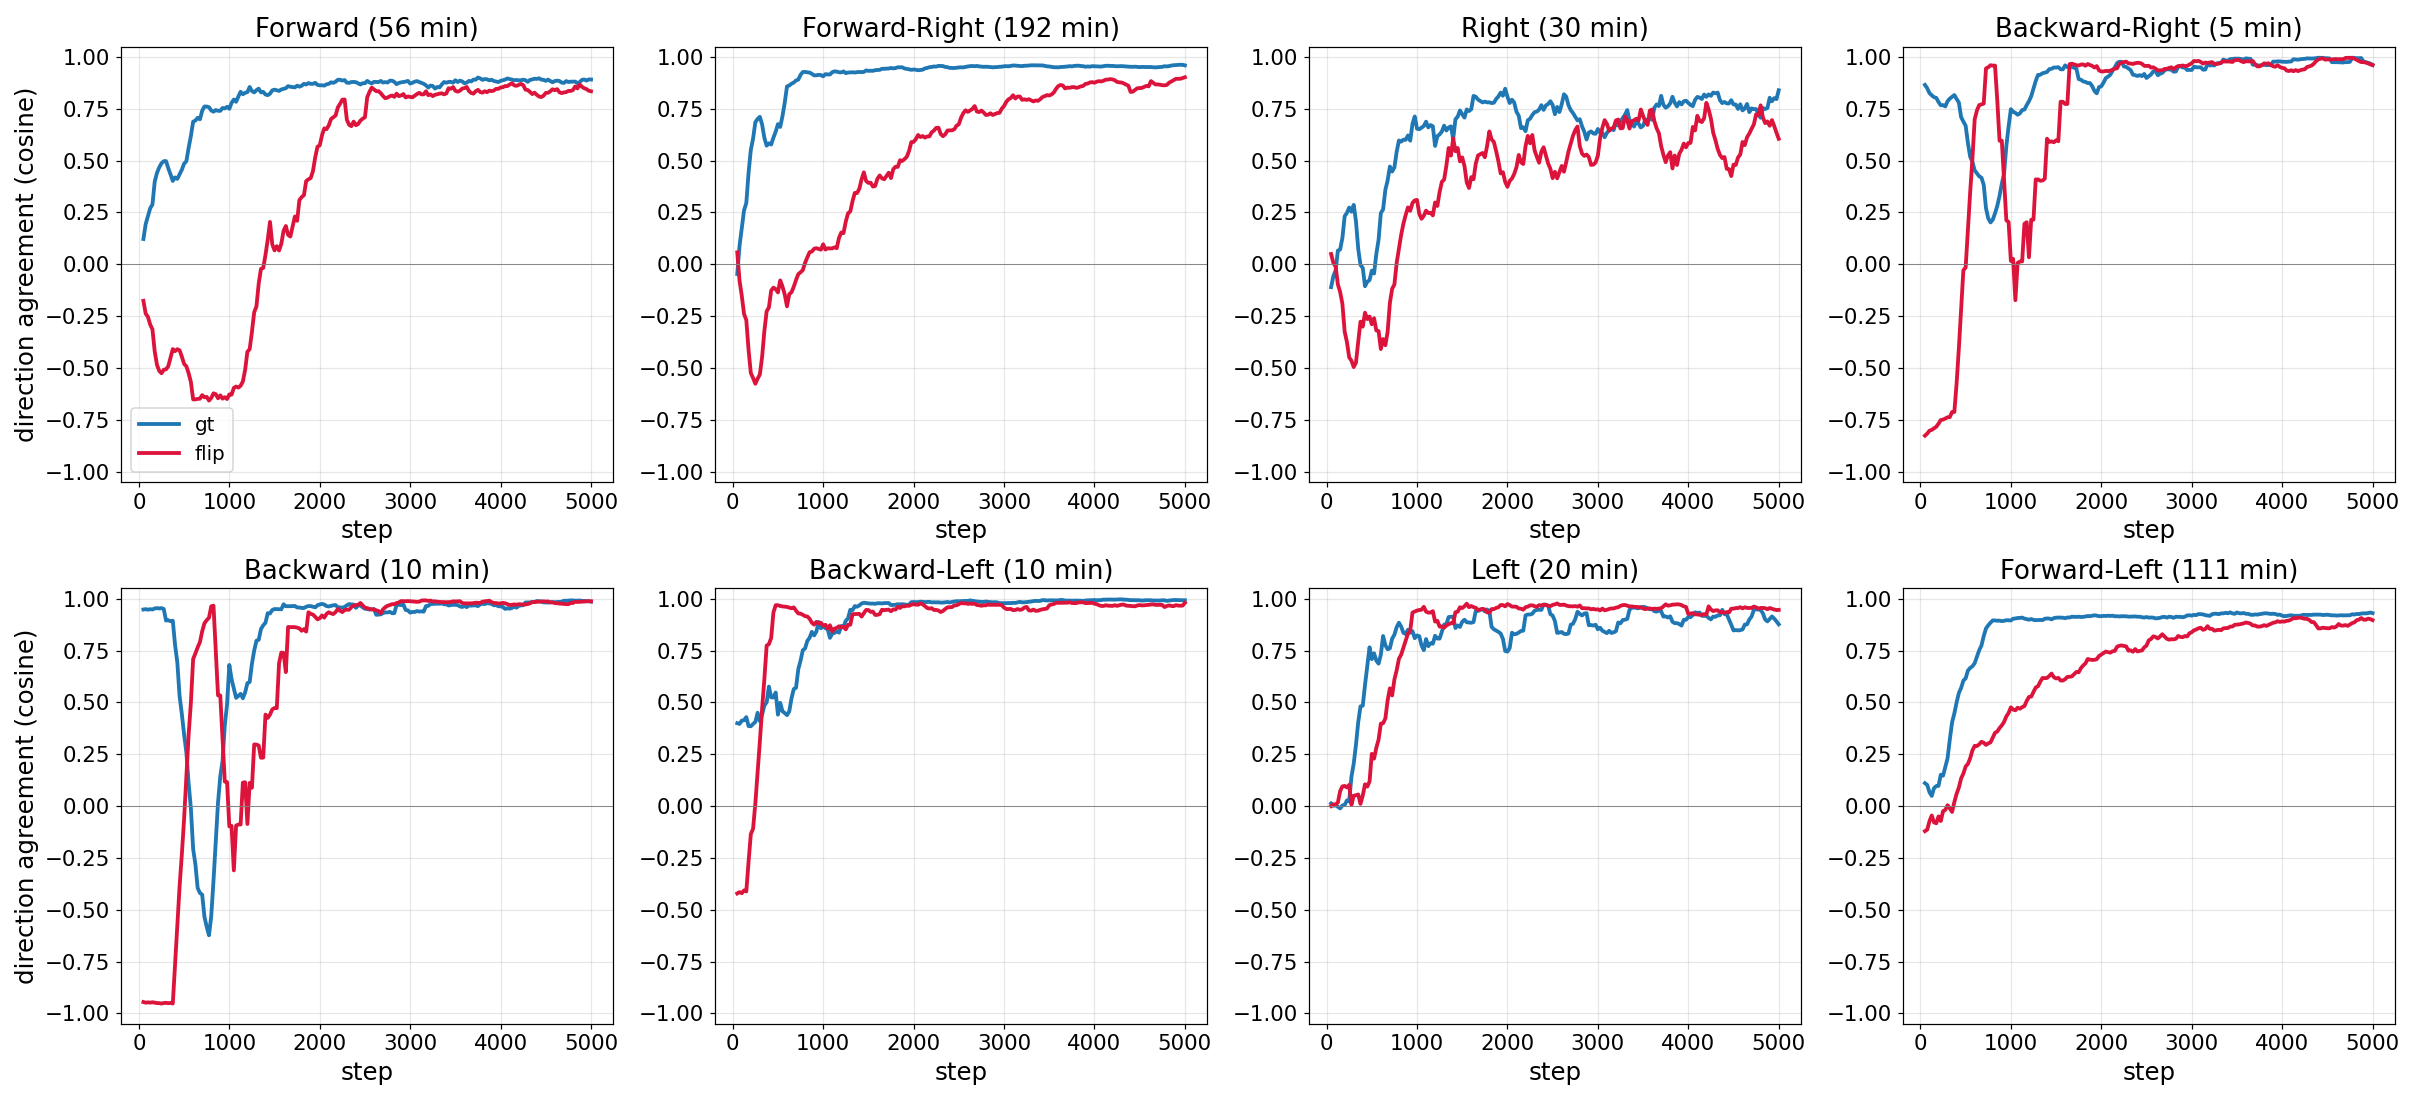
\includegraphics[
        width=0.82\textwidth
    ]{Figures/following_16node_by_REALdir.png}
    \caption{
        GT and FLIP agreement for the Batch64 model. FLIP becomes positive across
        all eight directions, demonstrating genuine command response. Panel titles
        denote source-context motion.
    }
    \label{fig:following_16pca}
\end{figure*}


\subsection{Batch-Size and Critic-Supervision Ablations}
\label{app:control_training_ablations}

Reducing either global batch size
(Fig.~\ref{fig:abl_nodes}) or the number of PCA components supervised by the
critic (Fig.~\ref{fig:abl_encoders}) delays convergence and weakens the
realized reverse response, but does not prevent recovery of the backward
direction. Every functional conditioning variant recovers backward control by
step $5{,}000$; only the tokens-only model fails. The corresponding effects on
generation quality are reported in
Appendix~\ref{app:quality_ablations}.

\begin{figure*}[t]
    \centering
    
\includegraphics[
        width=0.82\textwidth
    ]{Figures/following_FAMILY_nodes_by_REALdir.png}
    \caption{
        Batch-size ablation using global batch sizes $16$, $32$, and $64$
        under FLIP evaluation. All batch sizes recover the same directional
        structure by step $5{,}000$, but larger batches acquire the hardest
        throttle responses earlier and retain stronger reverse motion.
    }
    \label{fig:abl_nodes}
\end{figure*}

\begin{figure*}[t]
    \centering
    
\includegraphics[
        width=0.82\textwidth
    ]{Figures/following_FAMILY_encoders_by_REALdir.png}
    \caption{
        Critic-supervision ablation using the leading $2$, $4$, or $8$ PCA
        components. Two supervised components suffice to recover directional
        control, while richer supervision improves convergence and realized
        response strength.
    }
    \label{fig:abl_encoders}
\end{figure*}


\subsection{Settled Ablation Responses}
\label{app:settled_ablation_responses}

Figures~\ref{fig:wedge_g0} and~\ref{fig:wedge_g1} compare the settled
directional responses of the ablation variants. Batch size has its largest
effect on reverse throttle: Batch16 is substantially weaker under backward and
backward-diagonal commands than Batch32 and Batch64. Steering is less
sensitive to batch size and critic-supervision dimensionality, with every
functional variant retaining the expected signed four-lobe structure. The
tokens-only model fails to organize either action axis.

\begin{figure*}[t]
    \centering
    
\includegraphics[
        width=0.82\textwidth
    ]{Figures/wedge_g0.png}
    \caption{
        Settled throttle response $g_0$ by commanded direction for the ablation
        variants. Each translucent wedge represents one of $256$ rollouts; blue
        denotes realised forward motion and red realised backward motion. Solid
        outlines show medians, and panel rims show the local $95$th percentile. The
        tokens-only model renders every command as forward motion.
    }
    \label{fig:wedge_g0}
\end{figure*}

\begin{figure*}[t]
    \centering
    
\includegraphics[
        width=0.82\textwidth
    ]{Figures/wedge_g1.png}
    \caption{
        Settled steering response $g_1$ by commanded direction for the ablation
        variants. Blue denotes realised rightward yaw and red realised leftward yaw;
        opacity, outlines, and panel normalization otherwise follow
        Fig.~\ref{fig:wedge_g0}. Every functional variant shows the expected
        four-lobe structure.
    }
    \label{fig:wedge_g1}
\end{figure*}


\subsection{Cross-Model Response Curves}
\label{app:cross_model_response}

Figure~\ref{fig:response_gain_all} provides a scalar view of the behavior
summarized by the main-paper directional wedges. The curve construction and
uncertainty estimates are defined in
Section~\ref{app:response_details}.

Our model supports continuous-valued actions, whereas several baselines expose
only fixed pose increments, binary controls, or text commands without a
numerical strength parameter; see
Section~\ref{app:baseline_controls},
Table~\ref{tab:matrix_game_commands}, and
Table~\ref{tab:yume_commands}. Baselines are therefore shown only at strengths
supported by their released interfaces, and unsupported intermediate values
are not interpolated.

Because the interfaces use different and often non-metric units, the curves
are interpreted primarily through response sign and within-model
forward--backward asymmetry rather than absolute cross-model gain.

\begin{figure}[t]
    \centering

    \begin{subfigure}[t]{\columnwidth}
        \centering
        
\includegraphics[
            width=0.82\linewidth
        ]{Figures/response_curves_eval_throttle.png}
        \caption{Throttle response.}
        \label{fig:response_eval_forward}
    \end{subfigure}

    \begin{subfigure}[t]{\columnwidth}
        \centering
        
\includegraphics[
            width=0.82\linewidth
        ]{Figures/response_curves_eval_steer.png}
        \caption{Steering response.}
        \label{fig:response_eval_steer}
    \end{subfigure}

    \caption{
        Cross-model action-forcing response curves from $32$ low-egomotion
        held-out contexts. Realized motion is measured using the common
        CoTracker--PCA readout, and shaded bands show $\pm1$ SEM. Baselines are
        shown only at strengths supported by their released interfaces.
        The dotted diagonal denotes unit gain as a visual reference.
    }
    \label{fig:response_gain_all}
\end{figure}

\subsection{Cross-Model Steering and Yaw--Roll Coupling}
\label{app:cross_model_steering_roll}

Figure~\ref{fig:wedge_all_g1} shows that every evaluated model recovers the
requested steering sign, although response magnitude and consistency across
scenes differ. Figure~\ref{fig:wedge_all_g6} measures the roll-like component
$g_6$, which is not directly commanded but responds systematically to yaw
across several models.

A non-zero $g_6$ response is not necessarily a failure. Real egocentric turns
are rarely pure yaw rotations: vehicle dynamics, suspension, camera mounting,
and body motion can introduce a correlated roll component. Because the PCA
basis is recovered from real video, $g_6$ may capture this naturally coupled
motion. We therefore use it as a diagnostic of yaw--roll coupling rather than
assuming that all roll should vanish. Large or inconsistent responses remain
undesirable, particularly when they exceed the coupling observed in real
motion.

\begin{figure*}[t]
    \centering
    
\includegraphics[
        width=0.82\textwidth
    ]{Figures/wedge_all_g1.png}
    \caption{
        Steering response $g_1$ by commanded direction for all models. Blue denotes
        realised rightward yaw and red realised leftward yaw; other wedge
        conventions follow the main-paper throttle figure. Every model recovers the
        expected steering sign, although response magnitude and variance differ.
    }
    \label{fig:wedge_all_g1}
\end{figure*}

\begin{figure*}[t]
    \centering
    
\includegraphics[
        width=0.82\textwidth
    ]{Figures/wedge_all_g6.png}
    \caption{
        Uncommanded roll response $g_6$ under each planar command. Radius indicates
        roll magnitude; blue denotes clockwise and red counter-clockwise motion.
        Direction-dependent responses reveal coupling between commanded planar
        motion and out-of-plane camera motion.
    }
    \label{fig:wedge_all_g6}
\end{figure*}


\section{Reference-Free Quality Evaluation Methodology}
\label{app:quality_metrics}

Action-forced rollouts do not admit a unique ground-truth continuation, making
paired reference metrics unsuitable. We instead evaluate complementary
failure modes that can be measured without a target video: visual style shift, geometric corruption, scene relocation, conjuration (spurious object appearance), and progressive loss of high-frequency detail. This section defines the evaluation population,
inputs, scoring rules, thresholds, and validation procedure for each
instrument.


\subsection{Evaluation Population}
\label{app:quality_population}

The complete action-forcing benchmark contains $32\times8=256$ directional
rollouts per model. Two source contexts are unsuitable for feature-dependent
evaluation because water droplets and lens smearing leave their reference
frames nearly featureless. ORB detects only $371$ and $104$ keypoints in these
contexts, compared with approximately $2{,}900$--$3{,}000$ in representative
clean contexts. Reliable ORB--RANSAC correspondence counts are therefore
undefined for rollouts seeded from either context.

We exclude these two contexts uniformly from feature-dependent analyses. This
removes $2\times8=16$ rollouts from every model, leaving a common
$240$-rollout feature-valid population. The exclusion is a property of the
shared source footage rather than a model failure, and exactly the same
contexts and commands are removed for every model.

A model may avoid visible generation failures by producing little or no
motion. Within the feature-valid population, we therefore identify
near-static rollouts using the ORB matching and homography-verification
pipeline defined in Section~\ref{app:scene_relocation}. A rollout is classified
as static when its first generated frame and six-second-horizon frame retain
more than $600$ RANSAC-verified feature matches.

Style shift, scene relocation, and the deployed high-frequency-degradation
rate are reported on the model-specific active population, defined as
feature-valid and non-static. Geometry and conjuration do not require a
feature-rich reference and are therefore reported over all $256$ directional
rollouts. The resulting feature-valid and active populations are reported in
Table~\ref{tab:quality_denominators}.

\begin{table}[t]
\centering
{
\small
\begin{tabular}{lrr}
\toprule
Model or variant & Feature-valid & Active \\
\midrule
WorldPlay              & 240 & 238 \\
Matrix-Game            & 240 & 240 \\
WorldCam               & 240 & 216 \\
Astra                  & 240 & 215 \\
Yume                   & 240 & 237 \\
minWM                  & 240 & 187 \\
\midrule
Ours (Default)         & 240 & 239 \\
Ours (pca4)            & 240 & 237 \\
Ours (pca2)            & 240 & 232 \\
Ours (Batch 64)        & 240 & 237 \\
Ours (Batch 16)        & 240 & 236 \\
Ours (No Action Tokens)& 240 & 229 \\
Ours (No AdaLN)        & 240 & 200 \\
\bottomrule
\end{tabular}
}
\caption{
    Quality-evaluation populations. The complete directional fleet contains
    $256$ rollouts per model. Two wet-lens source contexts, corresponding to
    $16$ rollouts per model, are excluded uniformly because reference-based
    feature matching is undefined, leaving $240$ feature-valid rollouts.
    Active further excludes near-static continuations using the ORB-based
    criterion. Style, relocation, and deployed HF rates use the Active
    denominator.
}
\label{tab:quality_denominators}
\end{table}


\subsection{Geometric Corruption Probe}
\label{app:vlm_quality_probes}

We detect geometric corruption---melted, dissolving, or reality-breaking
structure---with a single binary probe implemented with Qwen3-VL-8B~\cite{QWEN}.
The probe receives one real reference frame followed by $16$ generated frames
distributed evenly over the available continuation, allowing it to assess
changes across the rollout rather than at a single time point.

The reference is frame $8$ of the shared real context. Generated-frame
selection is deterministic: the first and final available frames within a
six-second window are included, with the remaining frames placed uniformly
between them. The first
generated-frame indices are $9$ for ours, $4$ for Astra, $1$ for Matrix-Game,
$13$ for minWM, $65$ for WorldCam, and $1$ for WorldPlay and Yume as they are all designed to take different amounts of context. For our
$108$-frame rollouts, the selected indices are
$\{9,15,22,28,35,41,47,54,60,67,73,79,86,92,99,105\}$. Shorter baseline
rollouts are sampled over their available duration. All images are resized to
$640\times352$ and visibly labelled as \textsc{Reference} or
\textsc{Generated}.

The probe begins with the following preamble:

\begin{quote}
\small
\emph{The first image labelled REFERENCE is the last real frame of a driving
video---the true scene. The remaining images labelled GENERATED are an AI
world model's continuation of that exact scene, in temporal order. The model
was supposed to continue the SAME scene in the SAME visual style with
plausible content.}
\end{quote}

followed by the geometric-corruption question:

\begin{quote}
\small
\emph{Is there a SIGNIFICANT uncanny or reality-breaking failure in the
generated frames---impossible geometry, surfaces dissolving into abstract
patterns, large corrupted regions---that a casual viewer would notice within
one second? Ignore small local artifacts and minor blur. Answer Yes or No.}
\end{quote}

The question ends with the literal instruction
\texttt{Answer with ONLY \{"answer": "Yes"\} or \{"answer": "No"\}.}
The assistant response is force-prefixed with
\verb|{"answer": "|. No free-form text is decoded. The probe score is the
softmax probability of \emph{Yes} against \emph{No} at the next-token
position, and a rollout is flagged when $P(\mathrm{Yes})>0.5$.

\subsection{Style-Shift Instrument}
\label{app:style_instrument}

Style shift is a change in rendering rather than in content, so we measure it as
drift in a self-supervised feature space that responds to texture and rendering
statistics rather than to scene layout. We embed frames with
DINOv2 ViT-S/14~\cite{dinov2}: each frame is resized to $224\times224$ and
normalized with the standard ImageNet mean and standard deviation.

Two windows are compared. The anchor window is the first $\min(16,\text{ctx})$
real context frames; the end window is the last $16$ generated frames within the
six-second horizon. Each frame is embedded, the embeddings are
$\ell_2$-normalized, and the normalized embeddings are averaged over the window,
giving a single vector per window, $\bar e_{\mathrm{anchor}}$ and
$\bar e_{\mathrm{end}}$. The style-drift score is
\[
\texttt{dino\_drift}
=
1-\cos\!\left(\bar e_{\mathrm{anchor}},\,\bar e_{\mathrm{end}}\right),
\]
so that a continuation re-rendered in a different visual register moves far in
embedding space and scores high even when the geometry it depicts is unchanged.
A rollout is flagged when its drift exceeds a fixed high-drift threshold; as with
the high-frequency measure this threshold is descriptive and is not tuned on the
labelled evaluation set. A rollout is flagged when its DINOv2 drift exceeds $0.72$. This fixed
high-drift threshold is descriptive and is not tuned on the labelled
evaluation set. Although DINOv2 does not itself require keypoint matching, we
apply the common feature-valid mask because severe wet-lens corruption also
makes embedding drift relative to the source frame uninterpretable.

We also evaluated a VLM style probe as a candidate---the geometric-corruption
probe of Section~\ref{app:vlm_quality_probes} re-asked under the identical
protocol, querying whether the rendering style departs from the reference
(becoming painted, game-like, cartoonish, oversaturated, or otherwise
re-rendered), with ordinary lighting and exposure changes excluded. It is scored
comparatively and further explored in Section~\ref{app:val_style}.

\subsection{Scene-Relocation Instrument}
\label{app:scene_relocation}

Scene identity is measured geometrically and using feature matching instead of with VLMs. Frames are
resized to $640\times352$, converted to grayscale, and processed using
\[
\texttt{cv2.ORB\_create(3000)}.
\]
Descriptors are matched using
\[
\texttt{BFMatcher(NORM\_HAMMING, crossCheck=True)}.
\]
Matching therefore uses brute-force Hamming distance with mutual cross-check;
no Lowe ratio test is applied.

Matches are geometrically verified using a single homography:
\[
\texttt{cv2.findHomography(src,dst,cv2.RANSAC,5.0)},
\]
where $5.0$ is the reprojection threshold in pixels. The verified-inlier
count is the sum of the returned RANSAC mask.

For each source scene, one joint sibling set is constructed from the
six-second-horizon end frame of every evaluated rollout: six external
baselines and seven ablation variants. The real reference is frame index $8$
from the shared source context.

For each rollout, we retain the largest number of RANSAC-verified ORB matches
obtained against either the real reference frame or the endpoint of any other
model generated from the same source scene. A rollout is classified as
relocated when this best match contains fewer than $50$ verified
correspondences.

Using the best match makes the test intentionally conservative: a continuation
is considered to remain in-scene whenever it agrees with at least one valid
view of the source scene, rather than requiring agreement with every sibling
rollout.

The static filter uses the same ORB, descriptor-matching, and homography
pipeline. It compares each rollout's first generated frame with its
six-second-horizon end frame and classifies the rollout as static when the
verified-inlier count exceeds $600$.


\subsection{Conjuration Instrument}
\label{app:conjuration_instrument}

A strange by-product of training on third-person video games is that there will always be an
actor in the foreground who is controlled via commands, with the camera view rotating around
them. Sometimes these models create such an actor even when the scene does not have one, and we
label these as videos with conjured objects present, as they seem to apparate as if by magic.

In real world footage new objects appear constantly and legitimately: they enter from the side of
the frame, they approach from the distance until they cross the detector's resolution limit,
and they emerge from behind occluders. Reporting any object new to the frame is therefore
useless, as it flags every rollout. Requiring in addition
that the object be confidently detected, born inside the central portion of the frame rather
than at its border, and still present at the end removes most of these, but only reaches $0.84$
AUC at $0.59$ precision. Because conjuration is uncommon, low specificity is especially
punishing: with a base rate of a few percent, even a small false-positive rate dominates the
flagged set.

The property unique to conjurings is that the object has no history but that it remains in the frame until the end. We therefore judge every object across the entire rollout.
Objects are detected on every frame and linked into tracks; a track is considered a candidate
only if it is born after the context boundary, is not near the left or right border in its
first half second, reaches high confidence (to the object detector), covers a minimum area (to avoid pixel noise), and is still present near
the end of the rollout. Surviving tracks are then tested for prior appearance in three ways.

The \emph{onset} is the pixel change at the birth box divided by the change over the whole
frame, so that the egomotion which moves every pixel is divided out and only a relative spike
counts; the ratio must exceed $5.0$.

The \emph{zoom probe} crops where the object is about to be, in the frames before it exists,
upscales and re-detects: a distant real car is a few pixels at native resolution and looks like
absence, but resolves into a confident vehicle when magnified, whereas empty ground stays empty
at any magnification. A re-detection confidence of $0.50$ or above counts as the object having
already been there.

The \emph{back-match} correlates the object's own settled patch into pre-birth frames at the box
its trajectory extrapolates to, catching partial occlusion reveals; a correlation of $0.65$ or
above likewise counts as prior appearance.

Detections come from RT-DETR R50~\cite{zhao2024detrs}, run over all classes at a low confidence
threshold so that the weak-detection tail is available to the prior-appearance tests, with
tracks linked from detections scoring at least $0.30$; only classes that can plausibly be
conjured are reportable (car, truck, bus, motorcycle, and a small number of rigid stationary
items). Each test is expressed as a signed margin from its threshold, and a rollout is flagged
when the smallest of the three is positive, so all three must be satisfied independently.


\subsection{High-Frequency Degradation Instrument}
\label{app:high_frequency_metric}

Some variants progressively lose contrast and fine image structure during
long rollouts. We measure this effect using the change in Laplacian variance,
a standard indicator of high-frequency image content.

For a temporal window \(W\), let
\[
L_r(W)
=
\frac{1}{|W|}
\sum_{t\in W}
\operatorname{Var}\!\left(\nabla^2 g_{r,t}\right),
\]
where \(g_{r,t}\) is the grayscale frame from rollout \(r\) at time \(t\).
The base window contains four frames beginning near \(t=1\)\,s, while the
end window contains eight frames sampled with stride two near the end of the
rollout.

The loss of high-frequency detail in rollout \(r\) is
\[
\Delta_r
=
L_r(W_{\mathrm{base}})
-
L_r(W_{\mathrm{end}}),
\]
so that larger positive values indicate a greater reduction in sharpness.

To account for scene difficulty and source-image quality, we express this
loss relative to the other models generated from the same source scene:
\[
\mathcal B_r
=
\Delta_r
-
\operatorname{median}_{s\in\mathcal S_r}\Delta_s,
\]
where \(\mathcal S_r\) is the sibling group for rollout \(r\). Positive
\(\mathcal B_r\) therefore indicates greater sharpness loss than the typical
continuation of the same scene, while negative values indicate better
retention of high-frequency detail.

Against the $13$ hazy rollouts among our $112$-rollout ablation set ($16$ scenes),
the continuous score achieves AUC $0.85$, compared with $0.82$ for dark-channel
rise and $0.64$ for contrast loss. To summarize the continuous score as a failure rate, we classify a rollout as
high-frequency degraded when $\mathcal B_r>150$. This fixed reporting
threshold was not optimized on the labelled evaluation set. The resulting
percentage is therefore a descriptive summary of the score distribution,
while the AUC evaluates the continuous metric independently of any particular
threshold. Dark-channel and contrast measurements are reported only as
alternative candidate metrics and do not contribute to this classification.

\paragraph{Evaluation population.}
The deployed high-frequency-degradation rate is reported on the model-specific
active population: rollouts must be feature-valid and non-static. The two
wet-lens contexts are excluded through the feature-valid mask, but no
additional sharpness-quantile exclusion is applied to the main cross-model
failure rates.

\section{Reference-Free Quality Evaluation Validation}
\label{app:quality_validation}

We validate all five quality instruments against human annotations. Style
shift, geometric corruption, scene relocation, and conjuration are validated
on shared or enriched labelled sets. High-frequency degradation is validated
separately on the ablation set, where positive examples are more concentrated,
and then evaluated on the active cross-model populations defined in
Section~\ref{app:high_frequency_metric}.

It should be noted that evaluating these rollouts qualitatively without a reference requires nuance and subtlety; which means that some rollouts will inevitably be wrongly evaluated, however this is an unavoidable consequence of such an evaluation process, and we leave further performance gains and ensembling approaches to future work.

\subsection{Geometric Corruption}
\label{app:val_geometry}

Egomotion models re-render scene geometry as the viewpoint changes, and their
characteristic failure is localized over-warping: a surface keeps plausible
colour and coarse shape while its internal structure melts, duplicates, or
becomes impossible. Whole-frame pixel and line-segment statistics miss this, so
we compared a VLM probe that judges melted or geometrically impossible structure
against a generative artifact segmenter (PAL4VST~\cite{pal}) and a melt-specific
VLM prompt evaluated on left/right crops. Each candidate was scored against $36$
human ``mangle'' labels on the $100$-rollout subset
(Table~\ref{tab:val_geometry}).

The VLM geometric-corruption probe agrees best with human judgement at $0.78$
AUC. PAL4VST is close ($0.77$) but redundant with it. We evaluated the same
probe across three open VLMs to confirm the choice of backbone: Qwen3-VL-8B is
strongest, ahead of InternVL3-8B and Cosmos-Reason1-7B
(Table~\ref{tab:val_geometry}). We therefore deploy the single Qwen3-VL probe
and flag a rollout when $P(\mathrm{Yes})>0.5$; combining it with the segmenter
improves AUC only within noise.

As shown in Figures~\ref{fig:val_geometry_external} and ~\ref{fig:val_geometry_internal}, the geometry / warping metric earns its keep but it classifies one of the scene relocated rollouts (yume\_r27) as clean, we note that this is because the metric does not find any geometry warping and it is not designed to identify scene relocation. This further necessitates separate axes controls.

\begin{figure*}[t]
    \centering
    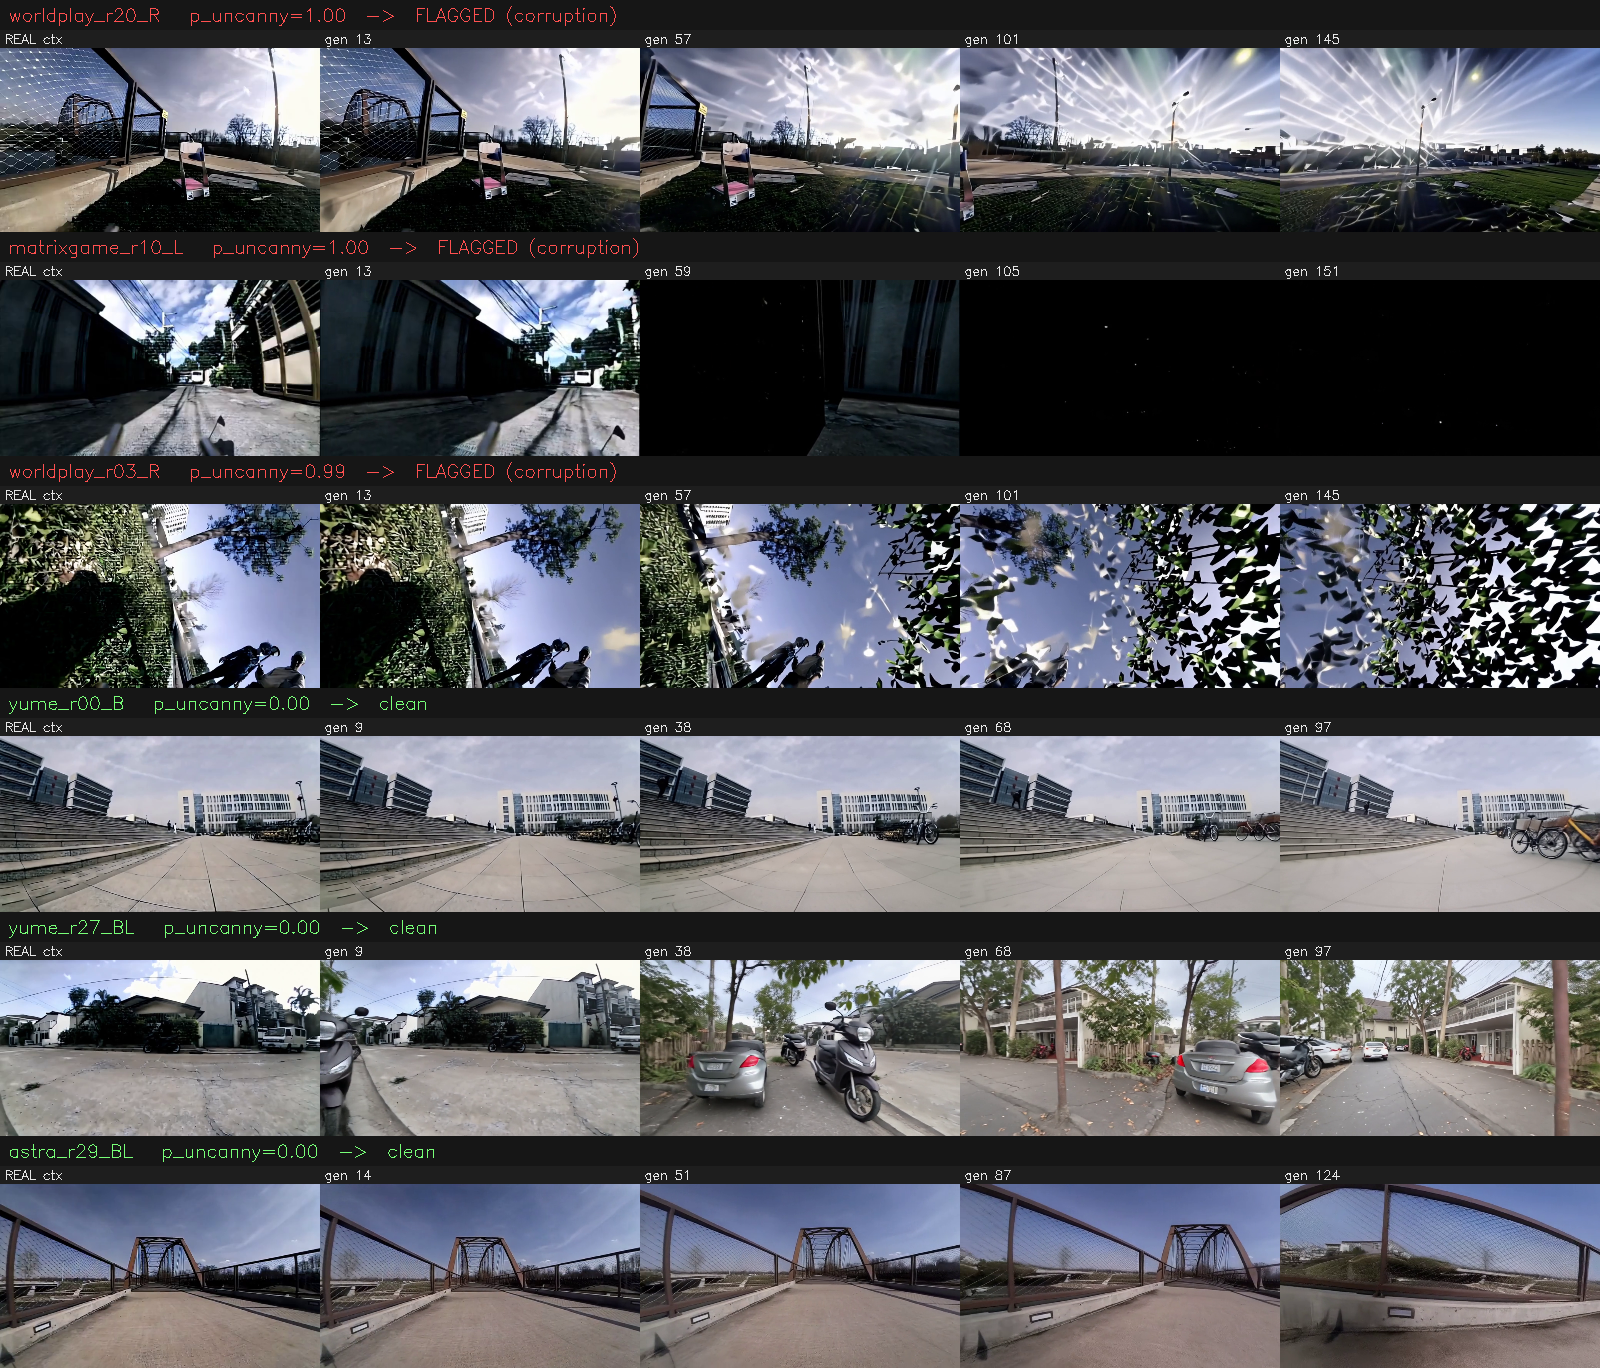
\includegraphics[
        width=0.82\textwidth
    ]{Figures/appendix_validation/geometry_validation_fleet_external.png}
    \caption{
        Geometry-instrument examples for the external baselines, showing
        representative human-positive and human-negative cases. Yume r27 is a false
        negative because it relocates without visible geometric corruption.
    }
    \label{fig:val_geometry_external}
\end{figure*}

\begin{figure*}[t]
    \centering
    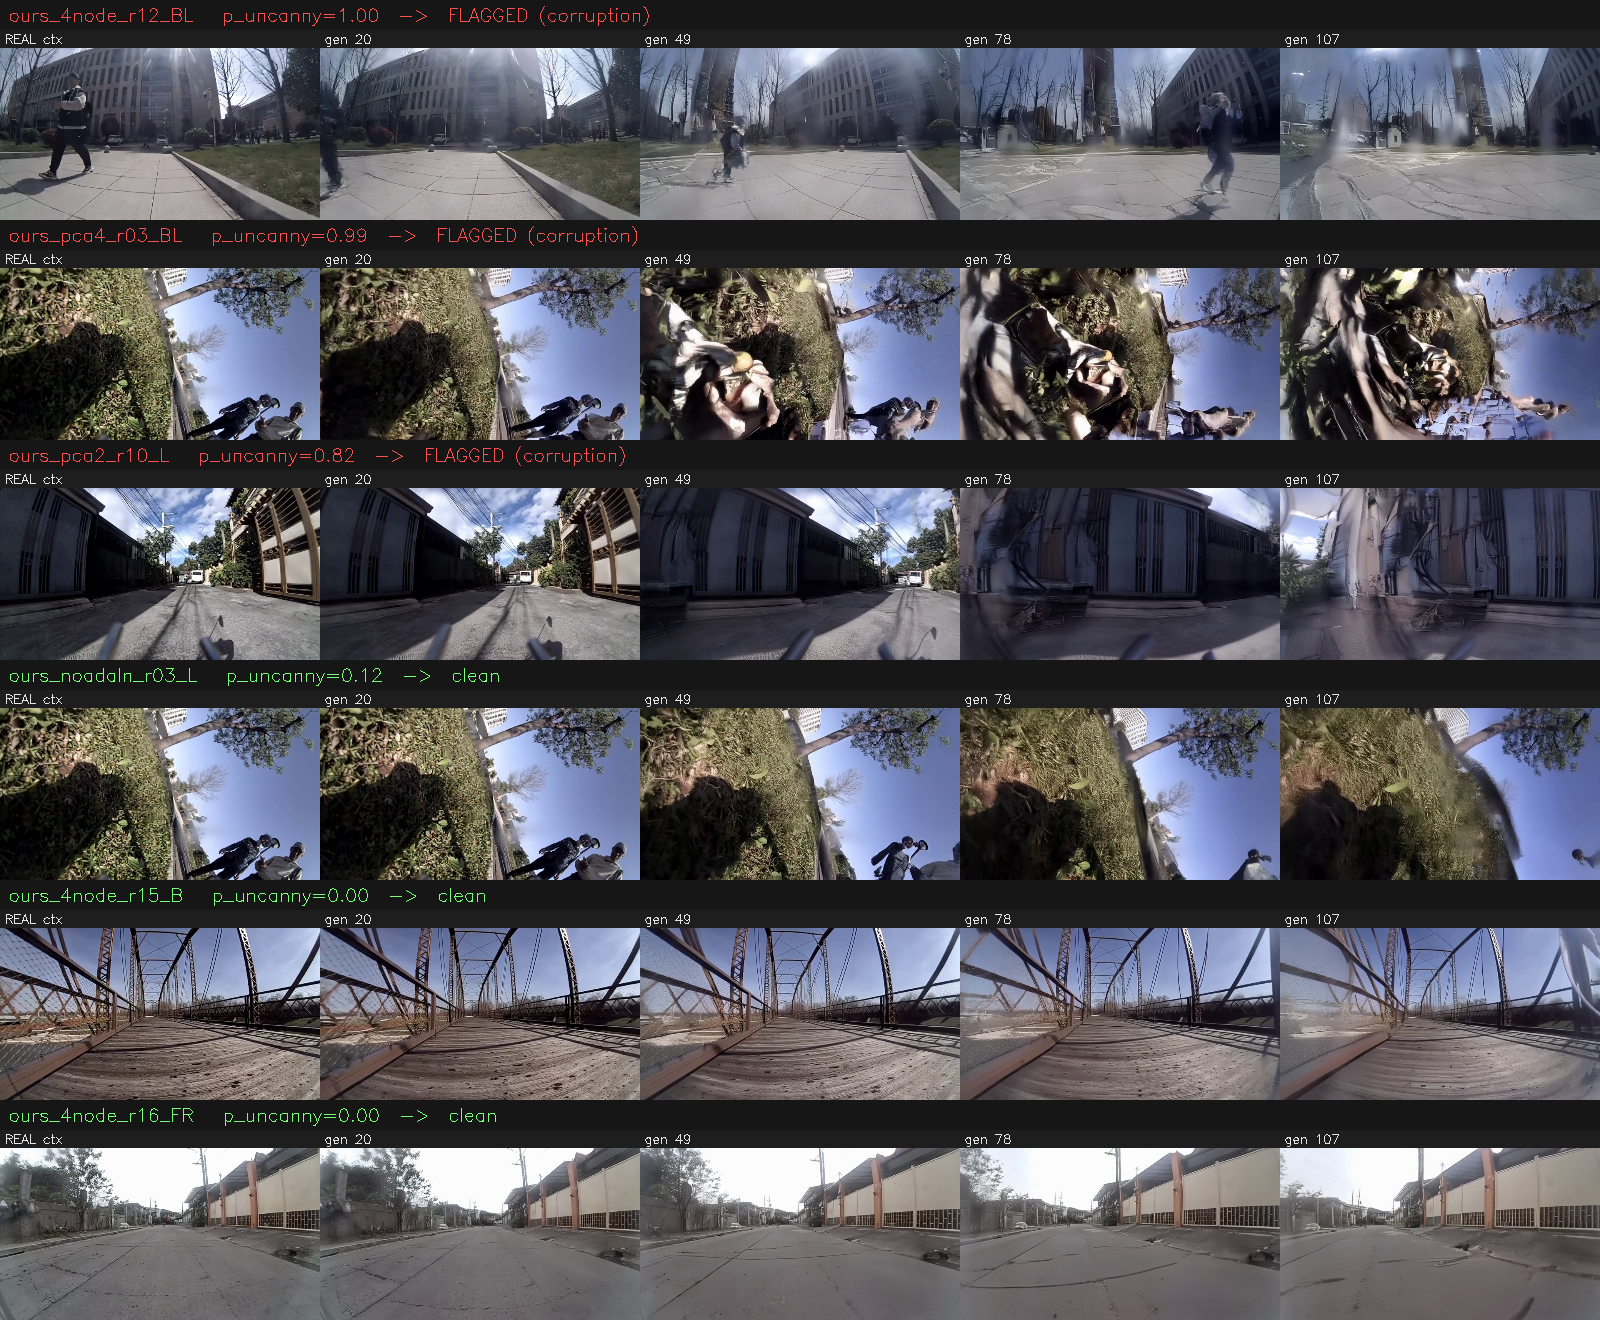
\includegraphics[
        width=0.82\textwidth
    ]{Figures/appendix_validation/geometry_validation_fleet_internal.png}
    \caption{
        Geometry-instrument examples for our ablation variants, showing
        representative human-positive and human-negative cases.
    }
    \label{fig:val_geometry_internal}
\end{figure*}

Table~\ref{tab:val_geometry} shows some competing techniques, we leave a more full analysis of these metrics and their ensembling methods to future work having highlighted the performance of such methods.

\begin{table}[t]
\centering
{
\small
\begin{tabular}{lc}
\toprule
Detector & AUC \\
\midrule
\textbf{VLM geometric-corruption probe (Qwen3-VL-8B)}
    & \textbf{0.78} \\
\quad same probe, InternVL3-8B
    & 0.75 \\
\quad same probe, Cosmos-Reason1-7B
    & 0.74 \\
PAL4VST artifact fraction
    & 0.77 \\
VLM melt probe, Cosmos-Reason1-7B
    & 0.71 \\
VLM melt probe, Qwen2.5-VL-7B
    & 0.68 \\
Depth-field curvature (Depth-Anything-V2)
    & 0.52 \\
\bottomrule
\end{tabular}
}
\caption{
    Geometric-corruption detectors scored against $36$ human mangle labels on
    the $100$-rollout subset. The deployed VLM probe (Qwen3-VL-8B) agrees best
    with human judgement; the same probe is evaluated across three open VLMs.
    The depth-curvature signal, part of an earlier ensemble, performs near
    chance ($0.52$) and is not used.
}
\label{tab:val_geometry}
\end{table}

\subsection{Style Shifts}
\label{app:val_style}

A style shift is a change in rendering rather than in content:
the continuation departs from the reference by becoming painted, game-like,
cartoonish, oversaturated, or otherwise re-rendered in a different visual
register, while the underlying scene layout may stay the same.

We compared a DINOv2 embedding drift against a CLIP embedding distance, a direct
style probe evaluated across three open VLMs (Qwen3-VL-8B~\cite{QWEN},
InternVL3-8B~\cite{internvl3}, and Cosmos-Reason1-7B~\cite{cosmos2}), and a
classical VGG Gram-matrix style distance~\cite{gatys2016image}, scoring each against
$20$ human style labels on the $100$-rollout subset
(Table~\ref{tab:style_metric_auc}). DINOv2 drift agrees best with human judgement
at $0.72$ AUC: the VLM probes asked directly whether the rendering changed land
lower and disagree with one another ($0.55$--$0.67$), the CLIP distance is close
but weaker ($0.70$), and the Gram-matrix distance is near chance. We therefore
deploy DINOv2 drift.

\begin{table}[t]
\centering
{
\small
\begin{tabular}{lc}
\toprule
Signal & AUC \\
\midrule
\textbf{DINOv2 embedding drift (deployed)} & $\mathbf{0.72}$ \\
CLIP embedding distance                    & $0.70$ \\
Cosmos-Reason1-7B style probe              & $0.67$ \\
Qwen3-VL-8B style probe                    & $0.66$ \\
InternVL3-8B style probe                   & $0.55$ \\
VGG Gram-matrix distance                   & $0.55$ \\
\bottomrule
\end{tabular}
}
\caption{
    Candidate style-shift measures evaluated by AUC on the human-labelled set
    containing $20$ positives among $100$ examples.
}
\label{tab:style_metric_auc}
\end{table}

As Figures~\ref{fig:style_external} and~\ref{fig:style_internal}
show, changes in weather or lighting are classified as style shifts which is permissible depending on the definition of style. However, it should be noted that sudden weather changes are possible and plausible, but it takes nuance to judge whether the model is arbitrarily changing the weather or if it is done in a correct way, so we permit it here.

\begin{figure*}[t]
    \centering
    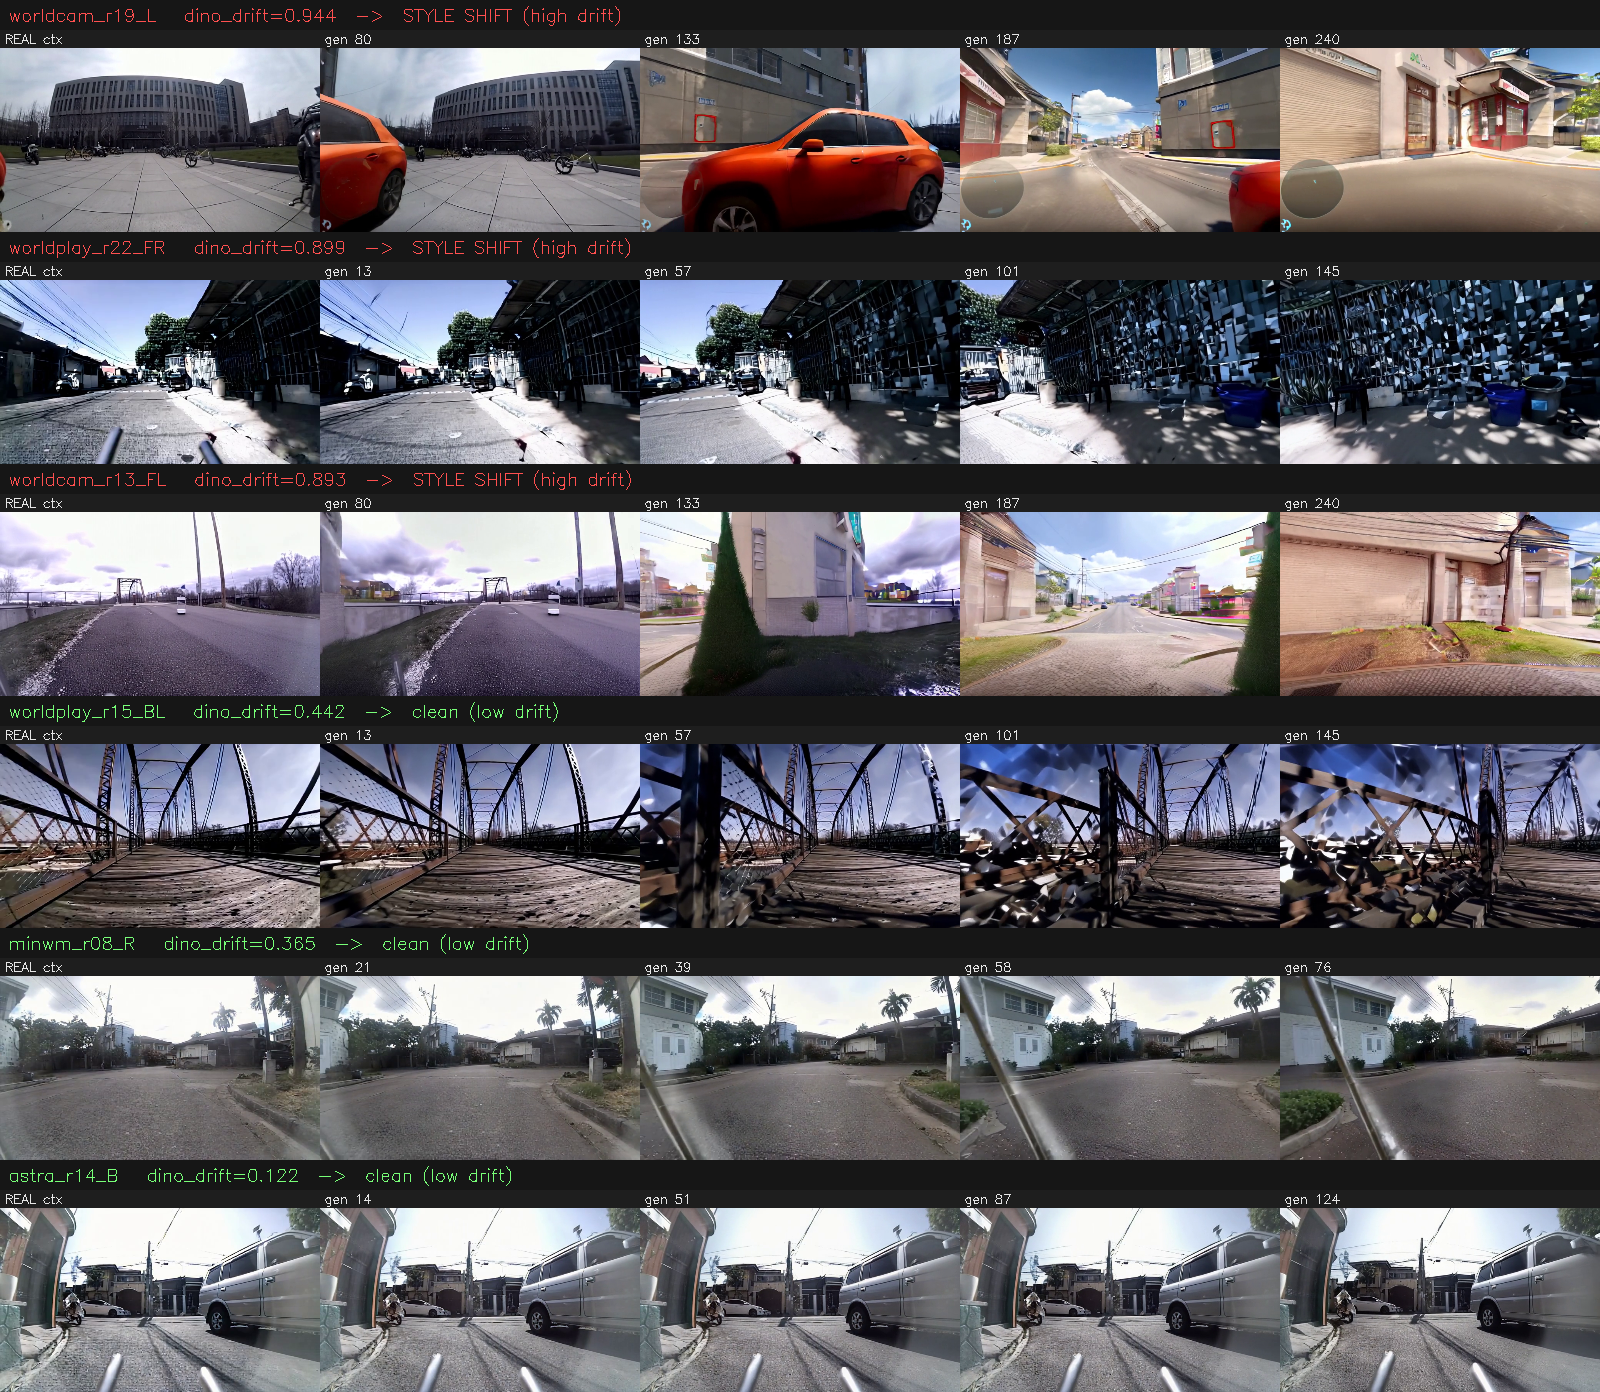
\includegraphics[
        width=0.82\textwidth
    ]{Figures/appendix_validation/style_validation_fleet_external.png}
    \caption{
        Style-shift-instrument examples for the external baselines, showing
        representative flagged and clean rollouts.
    }
    \label{fig:style_external}
\end{figure*}

\begin{figure*}[t]
    \centering
    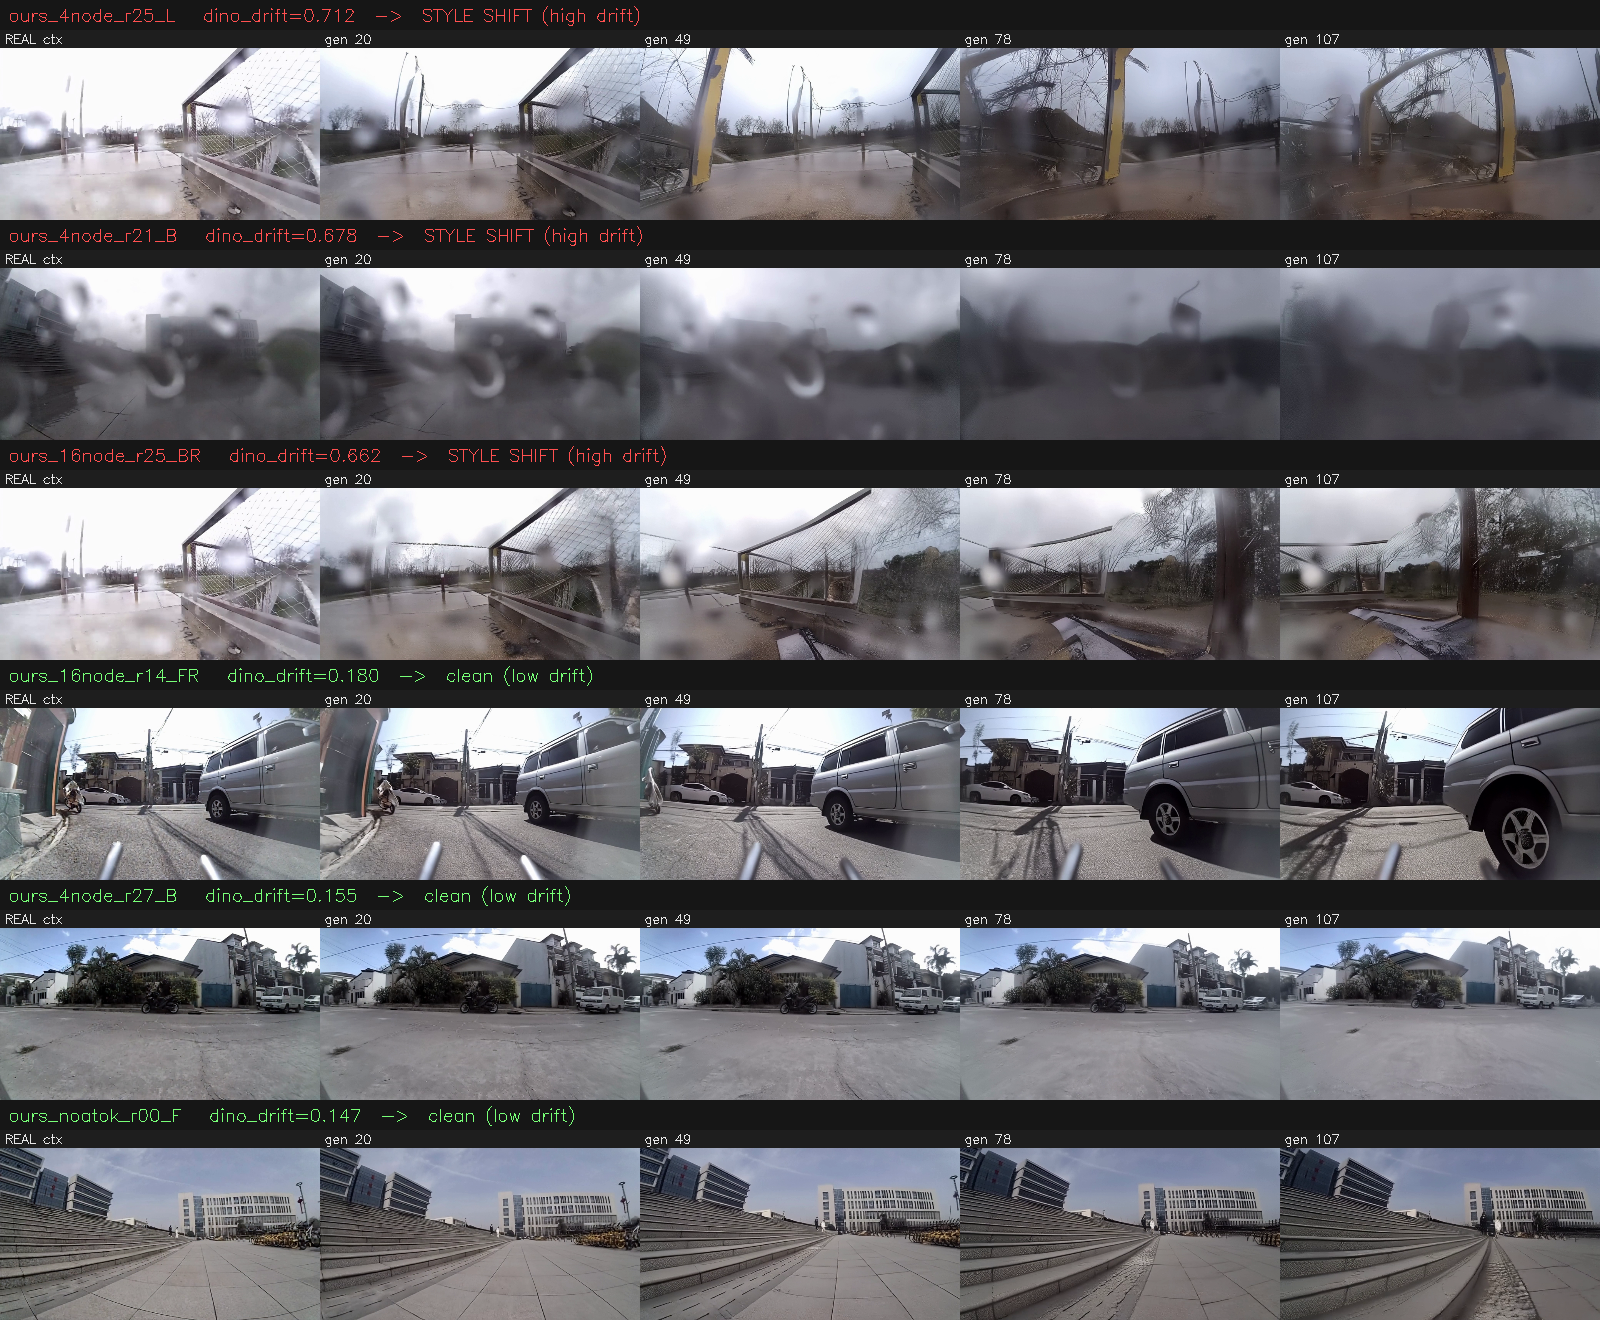
\includegraphics[
        width=0.82\textwidth
    ]{Figures/appendix_validation/style_validation_fleet_internal.png}
    \caption{
        Style-shift-instrument examples for our ablation variants, showing
        representative flagged and clean rollouts.
    }
    \label{fig:style_internal}
\end{figure*}

\subsection{Scene Relocation}
\label{app:val_scene}

A model can abandon the input scene and generate a plausible but different
place. We detect this geometrically rather than semantically: ORB keypoints are
matched between the generated six-second frame and the real reference, as well
as the end frames of sibling rollouts. A projective homography is fitted with
RANSAC, and the number of geometrically consistent inliers is counted. A
continuation that still depicts the same place retains many verified
correspondences, whereas a relocated continuation does not. A rollout is
flagged when fewer than $50$ geometrically verified inliers survive against
every available reference.

We compared feature detectors and embedding-drift alternatives against $19$
human relocation labels in a $100$-video subset
(Table~\ref{tab:val_scene}). Among classical detectors, ORB with RANSAC agrees
best with human judgement ($0.70$ AUC), ahead of AKAZE ($0.63$) and SIFT
($0.62$). RANSAC verification is important, as raw ORB matching drops to
$0.54$. DINOv2 embedding drift scores marginally higher ($0.72$), but provides
only a relative, uncalibrated distance. We deploy ORB+RANSAC because it yields
an absolute, interpretable per-rollout inlier count, requires no learned model,
and also serves as the static-rollout detector. The deployed fleet-consensus
pipeline uses a fixed threshold of $50$ verified inliers.

\begin{table}[t]
\centering
{
\small
\begin{tabular}{lc}
\toprule
Detector & AUC \\
\midrule
ORB + RANSAC inliers (deployed) & 0.70 \\
\textbf{DINOv2 embedding drift} & \textbf{0.72} \\
AKAZE + RANSAC inliers          & 0.63 \\
SIFT + RANSAC inliers           & 0.62 \\
ORB matches, no RANSAC          & 0.54 \\
\bottomrule
\end{tabular}
}
\caption{
    Scene-relocation detectors evaluated on a $100$-video human-labelled subset
    containing $19$ relocation positives. Higher AUC is better. ORB+RANSAC is
    deployed because it provides an absolute inlier count and also supports
    static-rollout detection.
}
\label{tab:val_scene}
\end{table}

Representative successes and failure cases are shown in
Figures~\ref{fig:scene_external} and~\ref{fig:scene_internal}.
Figure~\ref{fig:scene_internal} includes ambiguous flagged cases caused by
post-collision content and severe lens occlusion. Both can suppress geometric
correspondences without necessarily indicating true scene relocation. We retain
these rare edge cases rather than tune the detector specifically around them.

\begin{figure*}[t]
    \centering
    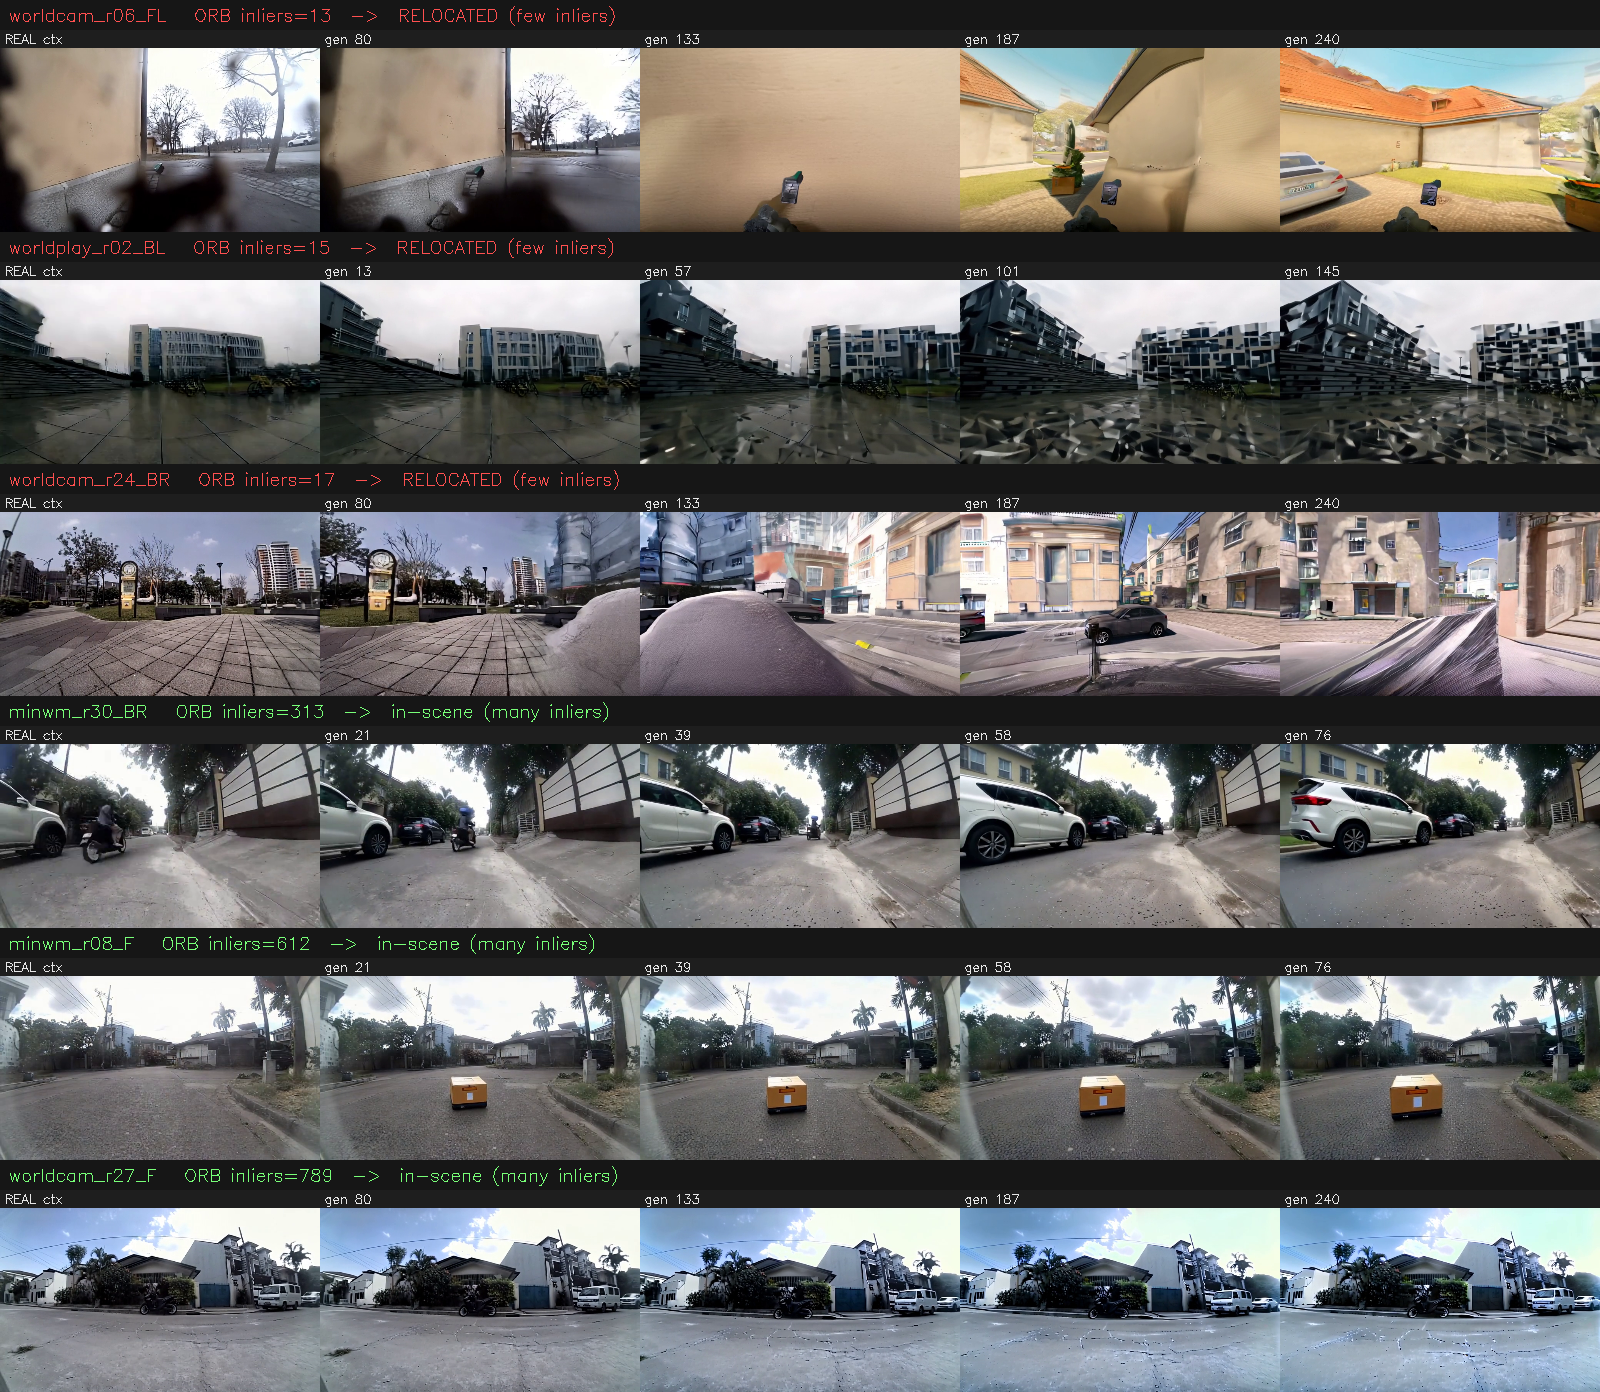
\includegraphics[
        width=0.82\textwidth
    ]{Figures/appendix_validation/scene_validation_fleet_external.png}
    \caption{
        Scene-relocation-instrument examples for the external baselines,
        showing representative relocated and retained-scene rollouts.
    }
    \label{fig:scene_external}
\end{figure*}

\begin{figure*}[t]
    \centering
    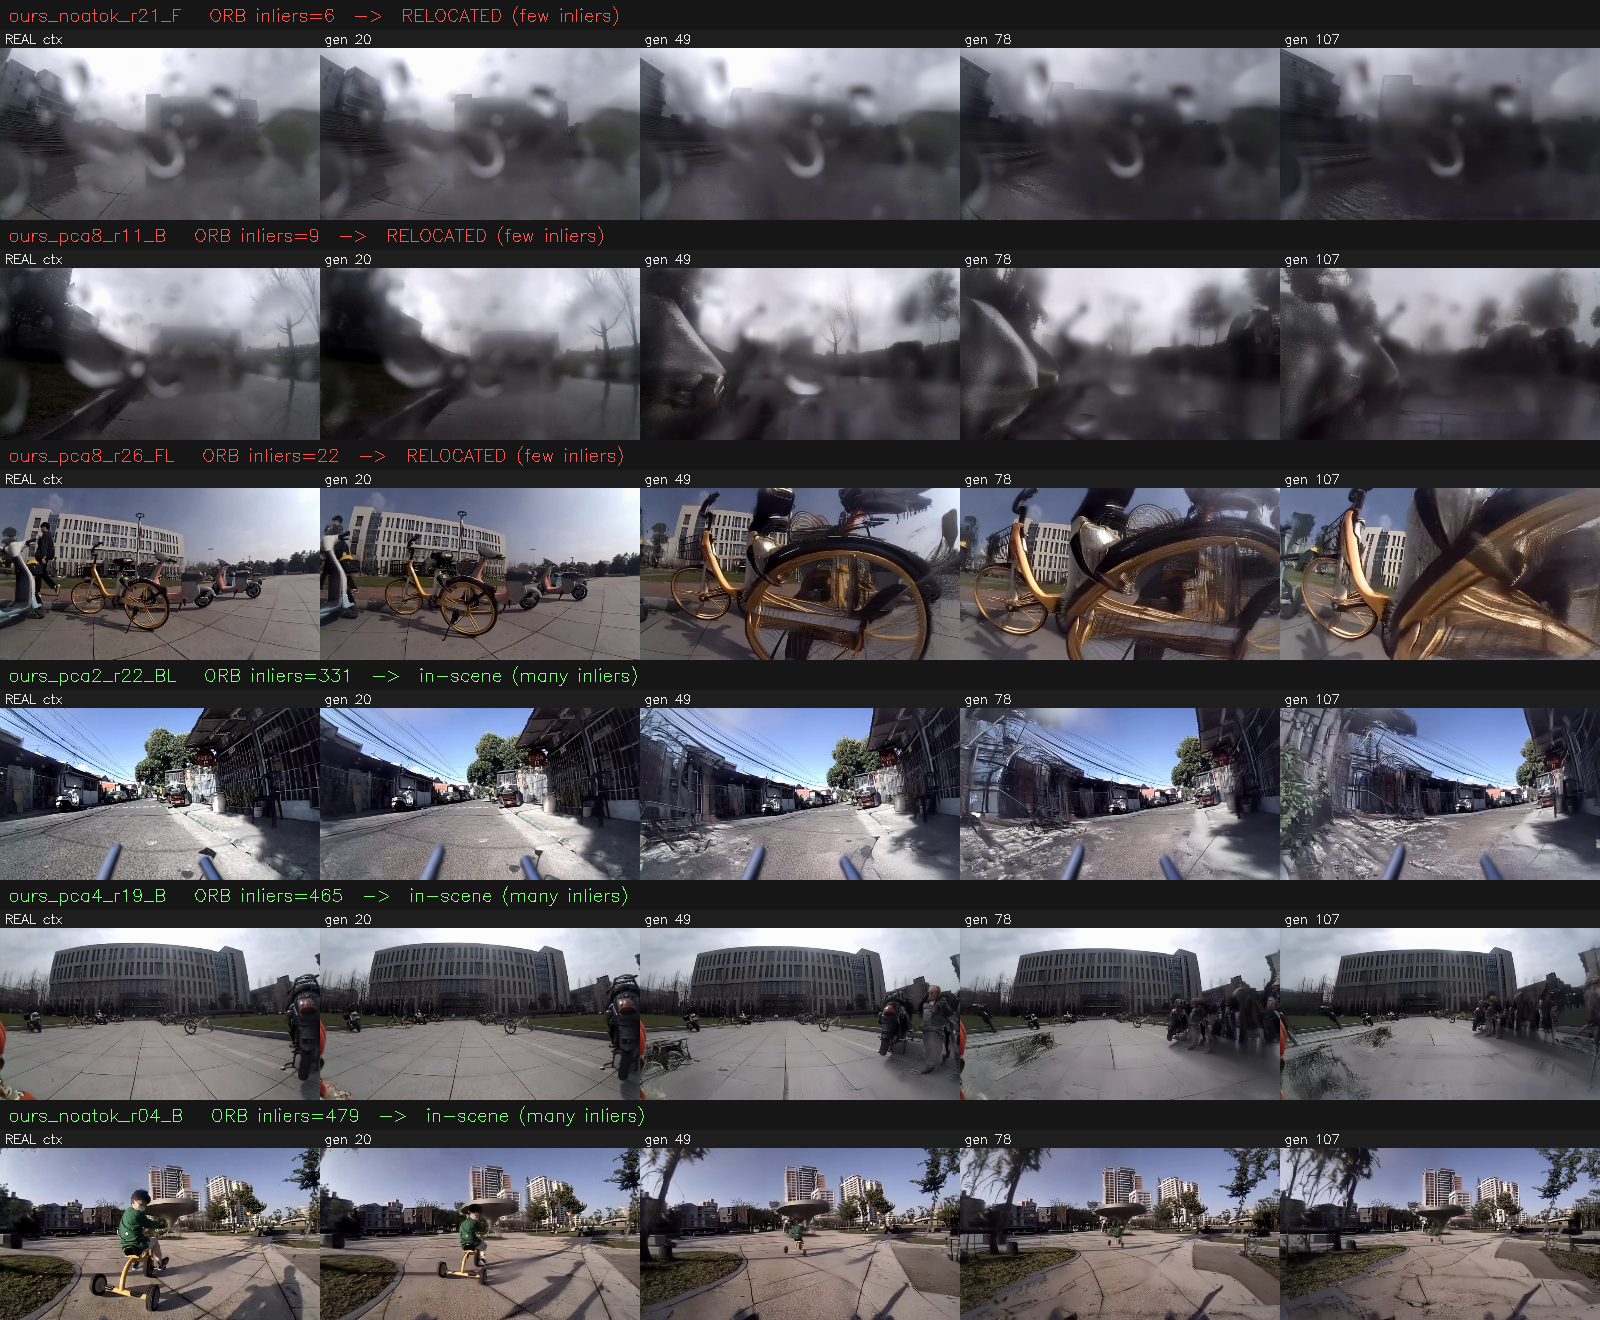
\includegraphics[
        width=0.82\textwidth
    ]{Figures/appendix_validation/scene_validation_fleet_internal.png}
    \caption{
        Scene-relocation-instrument examples for our ablation variants.
        Post-collision content and severe lens occlusion illustrate ambiguous
        flagged cases that suppress geometric correspondences without
        necessarily changing the underlying scene.
    }
    \label{fig:scene_internal}
\end{figure*}

\subsection{Conjuring}
\label{app:conj}

This is rare in our clips
and uncommon in most other baselines video, but certain models are prolific in it, so rather than reuse the
$100$-rollout subset (which contains too few positives to separate detectors) we assemble
a larger set enriched with true positives: $15$ confirmed
conjurations drawn from several models together with $22$ rollouts confirmed
clean, so that both precision and recall are measurable.

The temporal logic is agnostic to the detector backbone, so we validate that
choice across three architecturally distinct backbones under an identical
pipeline (Table~\ref{tab:val_conj}). RT-DETR and Faster R-CNN \cite{girshick2015fast}
are indistinguishable on this set---identical precision, recall and $F_1$, differing on no
rollout---so we deploy RT-DETR because it is $1.7\times$ faster. RetinaNet \cite{goyal2018focal}
loses one further rollout, and does so only because that rollout falls exactly on the decision
threshold rather than because it ranks it differently. The honest reading is that the backbone
barely matters and the temporal logic does the work.

\begin{table}[t]
\centering
{
\small
\begin{tabular}{lcccc}
\toprule
Backbone & Prec. & Rec. & $F_1$ & fps \\
\midrule
\textbf{RT-DETR R50 (deployed)} & 1.00 & 0.80 & 0.89 & \textbf{94.8} \\
Faster R-CNN R50-FPNv2          & 1.00 & 0.80 & 0.89 & 56.3 \\
RetinaNet R50-FPNv2             & 1.00 & 0.73 & 0.85 & 69.6 \\
\bottomrule
\end{tabular}
}
\caption{
    Detection backbones under an identical temporal pipeline, scored on the
    enriched evaluation set: $15$ confirmed conjurations drawn from several
    models together with $22$ rollouts confirmed clean, so that both precision
    and recall are measurable. Throughput is end-to-end detection plus temporal
    analysis on a single RTX 5090.
}
\label{tab:val_conj}
\end{table}

Figure~\ref{fig:conj_validation} shows the instrument at work: flagged rollouts
(top) have empty ground for the full second before the birth frame, after which a
crisp vehicle occupies it and persists; the clean rollouts (bottom) are the hard
cases a novel-object detector would fail on---a scooter present throughout, a
vehicle already in the scene, and a distant vehicle approaching---each annotated
with the test that rejected it.

\begin{figure*}[t]
    \centering
    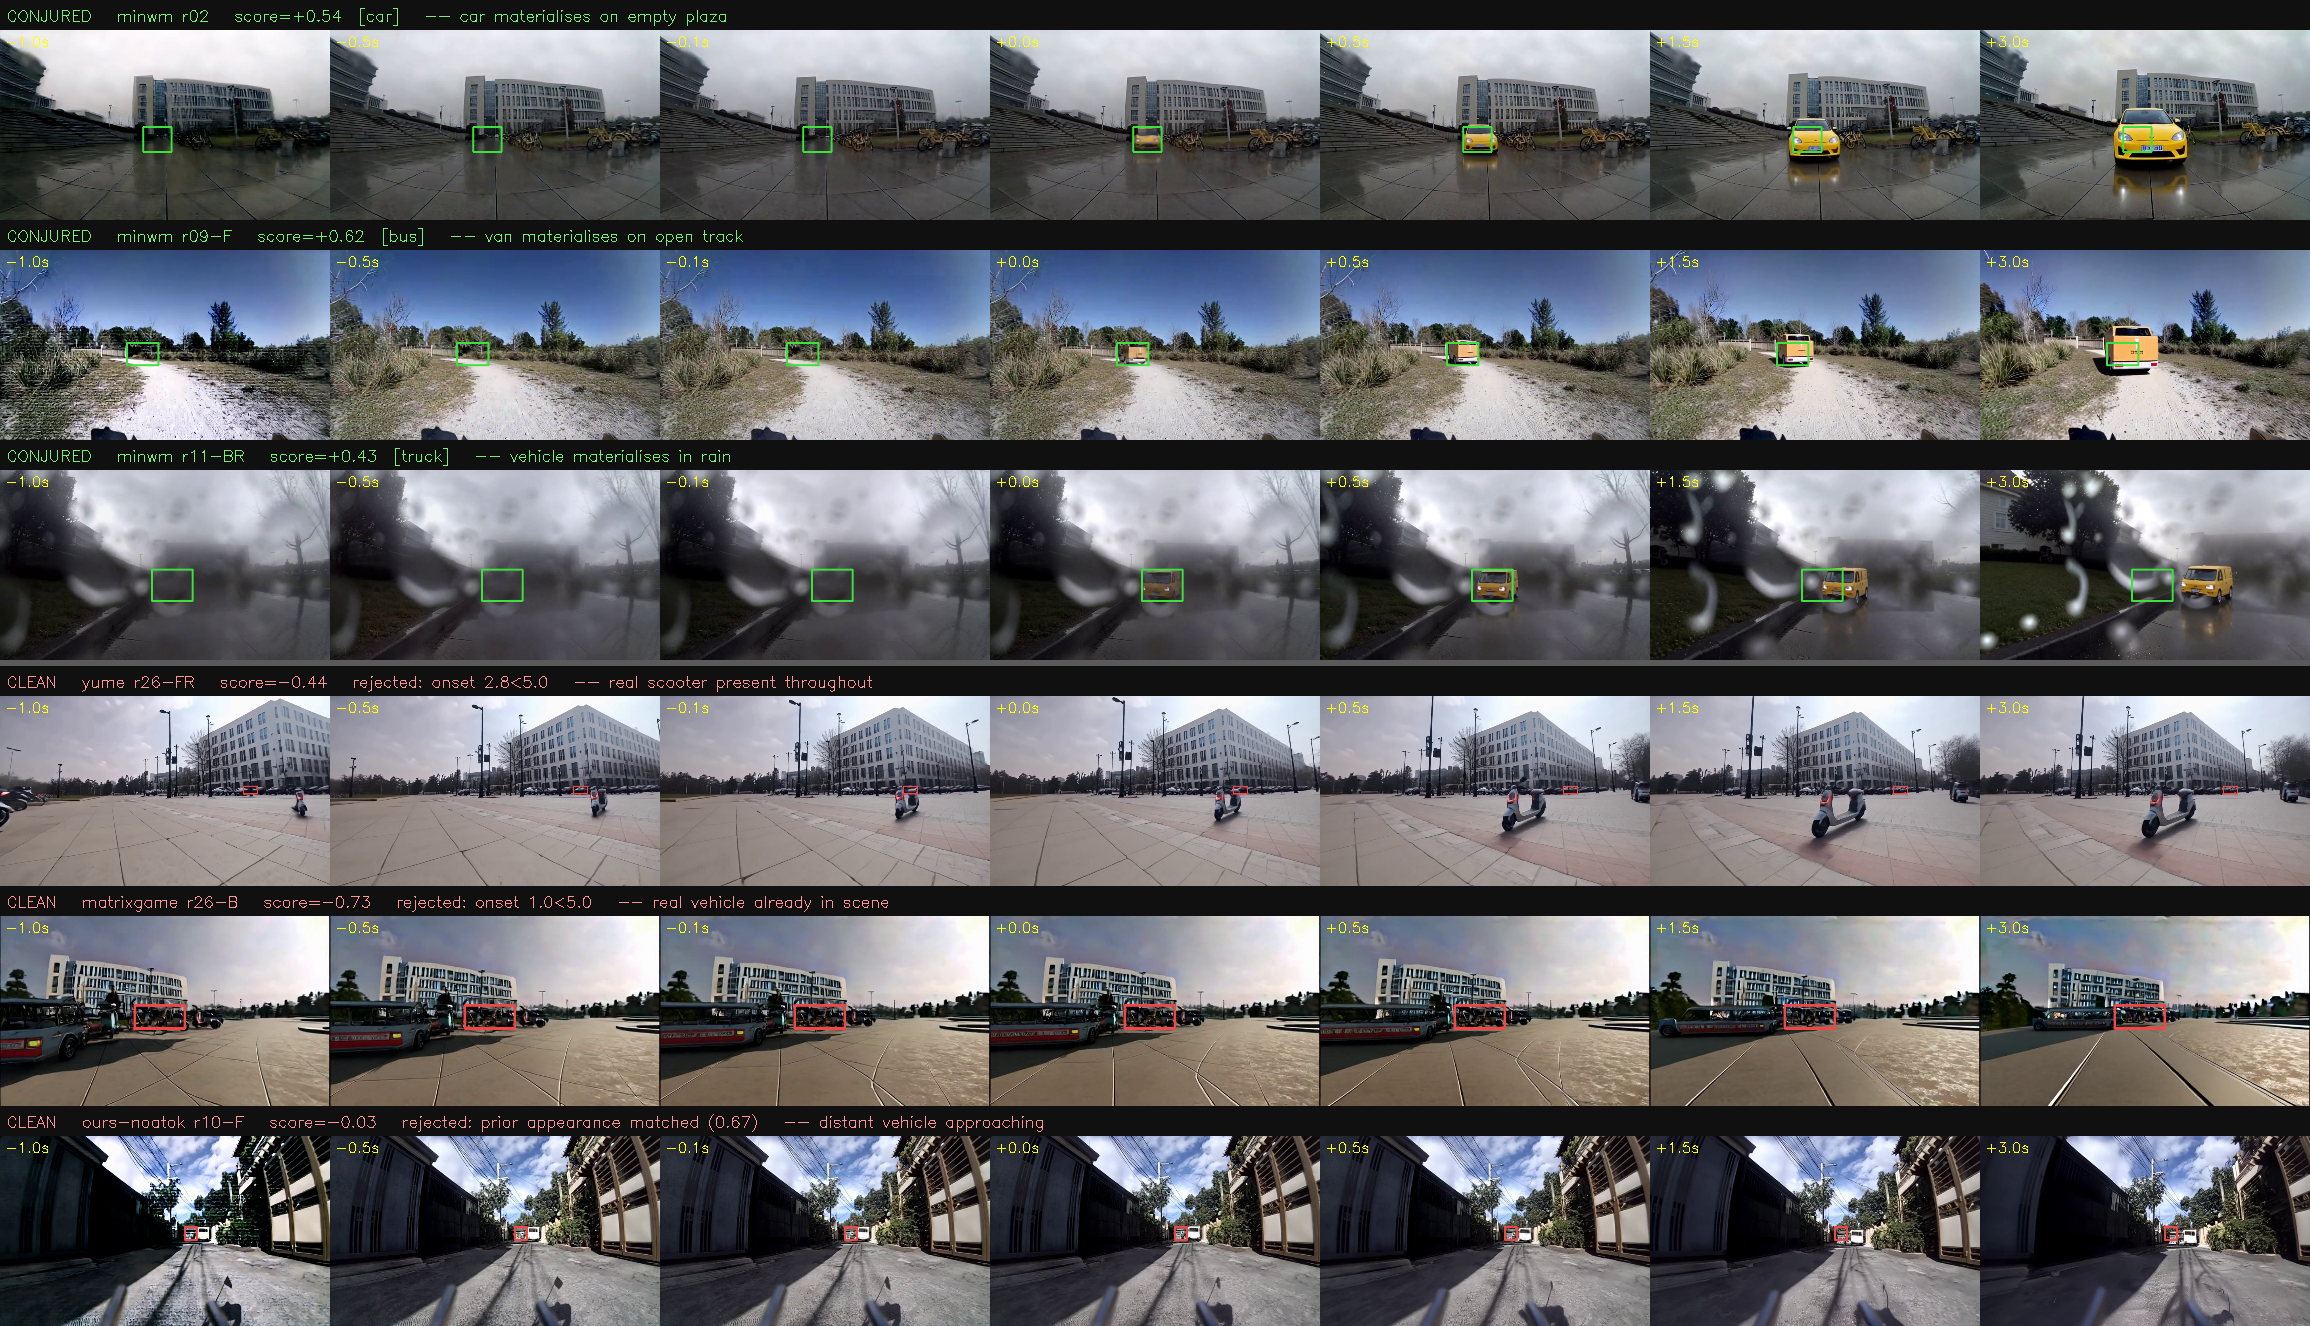
\includegraphics[width=0.82\textwidth]{Figures/appendix_validation/conjuring_validation.png}
    \caption{
        Conjuration-instrument examples. Top: flagged rollouts centred on object
        birth, showing empty ground beforehand and a persistent object afterwards.
        Bottom: hard negatives in which new objects arrive legitimately; annotations
        identify the prior-appearance test that rejected each candidate.
    }
    \label{fig:conj_validation}
\end{figure*}

What the instrument counts is narrower than ``any new object,'' deliberately: a
conjured object is a hallucination rather than a plausible arrival---rendered at
high resolution, crisper and more saturated than its surroundings, appearing
where nothing was and persisting for the rest of the rollout. Pedestrians,
cyclists, and other scene furniture are prevalent in generations and mostly
well behaved; conjured versions of these do occur with some models but through occlusion or the side of the frame, which is plausible and prevalent in real world video. Apparating out of thin air however is not present in any real world video so we classify this as a failure mode. 

Deployed over the full directional fleet, capped at six seconds of generation
per rollout, the instrument flags $2.1\%$ of rollouts. The rate is highly
non-uniform: minWM is flagged in $19.9\%$ of its rollouts, compared with
$0.84\%$ across our seven variants and $0.23\%$ across the other five external
baselines. Two controls indicate this reflects the model rather than the instrument. First,
the same scenes as real footage are flagged $0$ times out of $32$, so the detector does not
fire on genuine driving video. Second, and more telling, the gap is already present
\emph{before} any prior-appearance evidence is applied: minWM produces a persistent, crisp,
newborn interior object in $52.7\%$ of its rollouts, against $6.6$--$16.4\%$ for every other
model. The instrument is not simply more sensitive on minWM; minWM spawns far more new
persistent objects, and a sixth of its rollouts contain one that no prior-appearance test can
account for.

Whatever makes minWM the strongest baseline on
style, geometry and relocation renders it prone to inventing objects; perhaps slowly inventing objects leads to within distribution generation leading to stability.

\subsection{High-Frequency Degradation}
\label{app:val_hf}

High-frequency degradation is most pronounced in some of our ablations, so we
validate the instrument on the $16$ ablation scenes containing all seven
variants ($112$ rollouts), of which $13$ are human-labelled as degraded. After
validation, the same instrument and fixed reporting threshold are applied to
all internal and external models.

We compared the drift in Laplacian variance (a standard sharpness measure), the
drift in a dark-channel haze estimate, and the drift in global contrast, each
scored against those $13$ haze labels (Table~\ref{tab:val_hf}). Two design
choices matter and are validated by the table. First, the measure must be
\emph{baseline-aware}: some source clips begin hazy or blurred (water or smudge
on the physical lens), which is not a model failure, so we subtract the value
measured one second into generation and score only the subsequent change.

Second, each rollout is expressed relative to the median drift of its same-scene
siblings, which removes scene-dependent texture and difficulty. The
sibling-relative Laplacian-variance drift agrees best with human judgement at
$0.85$ AUC, ahead of the dark-channel haze drift ($0.82$); the raw,
non-sibling-relative variants and the contrast measure are markedly weaker
($0.64$--$0.77$). We therefore deploy the sibling-relative Laplacian-variance
drift and flag a rollout when it exceeds the descriptive threshold defined in Section~\ref{app:high_frequency_metric}. 

\begin{table}[t]
\centering
{
\small
\begin{tabular}{lc}
\toprule
Detector & AUC \\
\midrule
\textbf{Laplacian-variance drift, sibling-relative (deployed)}
    & $\mathbf{0.85}$ \\
Dark-channel haze drift, sibling-relative
    & $0.82$ \\
Dark-channel haze drift, raw
    & $0.77$ \\
Laplacian-variance drift, raw
    & $0.68$ \\
Contrast drift
    & $0.64$ \\
\bottomrule
\end{tabular}
}
\caption{
    High-frequency-degradation detectors scored against $13$ human haze labels
    on the $112$-rollout ablation set. The deployed measure is the change in
    Laplacian variance, expressed relative to same-scene siblings and net of the
    one-second baseline. The sibling normalisation and baseline subtraction are
    both necessary, as the raw variants show.
}
\label{tab:val_hf}
\end{table}

Figure~\ref{fig:hf_internal} shows representative rollouts to which the
high-frequency-degradation instrument is applied.

\begin{figure*}[t]
    \centering
    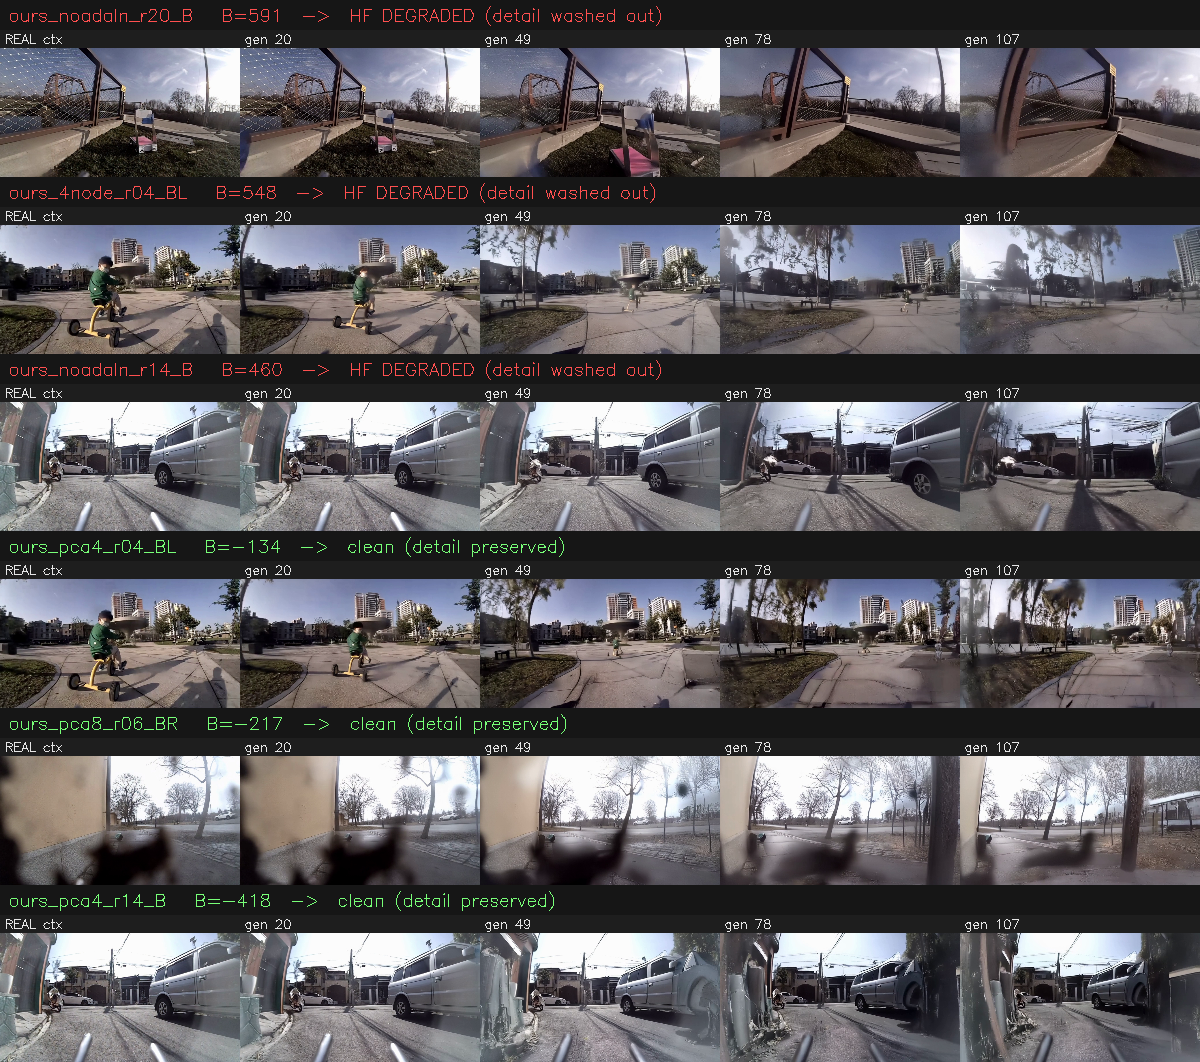
\includegraphics[width=0.82\textwidth]{Figures/appendix_validation/hf_validation_internal.png}
    \caption{
        The high-frequency-degradation instrument on our ablation variants. High-$B$
        rollouts (top) visibly wash out over the generated span---texture and contrast are
        lost by the end---while low-$B$ rollouts (bottom) preserve detail. The same source
        scenes appear in both classes, so the effect is model-dependent, not scene-dependent.
    }
    \label{fig:hf_internal}
\end{figure*}


\section{Quality Evaluation Results}
\label{app:quality_results}

We apply the reference-free instruments defined in
Section~\ref{app:quality_metrics} to the external baselines' generations and our ablation
variants' generations. We first compare quality failures across models and then examine how
the action-conditioning design, critic supervision, and training batch size
affect the failure profile of our model.

\subsection{Quality Ablations}
\label{app:quality_ablations}

Table~\ref{tab:quality_ablation} compares the quality-failure profiles of the
ablation variants. The default model provides the strongest overall balance,
with low style shift, geometric corruption, relocation, conjuration, and
high-frequency degradation. \texttt{Batch64} reduces relocation from $11\%$
to $9\%$, but increases geometric corruption from $17\%$ to $26\%$.

Reducing critic supervision to \texttt{pca4} and \texttt{pca2} raises
geometric corruption to $38\%$ and $40\%$, respectively, while
high-frequency degradation rises to $11\%$ and $22\%$. Reducing the
training batch size produces a different failure profile: relative to
\texttt{Batch64}, \texttt{Batch16} raises relocation from $9\%$ to $26\%$,
high-frequency degradation from $6\%$ to $43\%$, and geometric corruption
from $26\%$ to $32\%$. Removing the action tokens yields $29\%$
geometric corruption, $14\%$ relocation, and $20\%$ high-frequency
degradation.

The low geometric-corruption rate of \texttt{No AdaLN} should not be
interpreted as strong generation quality. This variant frequently produces
weak or unresponsive continuations and therefore introduces less new scene
structure that can become visibly corrupted. It nevertheless has the highest
relocation and high-frequency-degradation rates in the ablation grid.

\begin{table}[t]
\centering
{
\small
\setlength{\tabcolsep}{4pt}
\begin{tabular}{lccccc}
\toprule
Variant & Style\,\% & Geometry\,\% & Reloc.\,\% & Conjuring\,\% & HF\,\% \\
\midrule
Batch64          & $3$ & $26$ & $9$  & $0$   & $6$  \\
Default          & $3$ & $17$ & $11$ & $1$   & $6$  \\
pca4             & $3$ & $38$ & $13$ & $0$ & $11$ \\
pca2             & $3$ & $40$ & $15$ & $0$   & $22$ \\
Batch16          & $5$ & $32$ & $26$ & $1$ & $43$ \\
No Action Tokens & $3$ & $29$ & $14$ & $1$   & $20$ \\
No AdaLN         & $4$ & $11$ & $28$ & $2$ & $48$ \\
\bottomrule
\end{tabular}
}
\caption{
    Quality failure rates across the ablation grid; lower is better. Geometry
    and conjuration use all $256$ directional rollouts per variant. Style
    shift, relocation, and HF use the model-specific active populations in
    Table~\ref{tab:quality_denominators}. Geometry measures severe structural
    corruption. Relocation denotes fewer than $50$ RANSAC-verified matches to
    the real reference or any sibling end frame. Conjuring measures the abrupt
    introduction of new objects, style measures a change in rendering
    appearance, and HF measures progressive high-frequency degradation.
}
\label{tab:quality_ablation}
\end{table}

\subsection{High-Frequency Degradation}
\label{app:high_frequency_results}

Table~\ref{tab:hf_losses} reports the sibling-relative high-frequency
degradation score $\mathcal B$ defined in
Section~\ref{app:high_frequency_metric}.

The \texttt{Default} and \texttt{Batch64} variants remain stable, exceeding
the descriptive threshold $\mathcal B>150$ in $6\%$ and $6\%$ of active
rollouts, respectively. Reducing critic supervision to \texttt{pca4} and
\texttt{pca2} raises this rate to $11\%$ and $22\%$, while removing the
action tokens raises it to $20\%$.

The strongest degradation occurs under \texttt{Batch16} and
\texttt{No AdaLN}, which exceed the threshold in $43\%$ and $48\%$ of
active rollouts. Their positive median $\mathcal B$ values also indicate
systematic loss of high-frequency detail relative to sibling continuations
of the same scenes.

\begin{table}[t]
\centering
{
\small
\begin{tabular}{lrrr}
\toprule
Variant & Median $\mathcal B$ & $\mathcal B>150$ (\%) & $n/N$ \\
\midrule
Default          & $-108$ & $6$  & $14/239$  \\
Batch64          & $-78$  & $6$  & $15/237$  \\
pca4             & $-57$  & $11$ & $25/237$  \\
No Action Tokens & $+40$  & $20$ & $45/229$  \\
pca2             & $+47$  & $22$ & $52/232$  \\
Batch16          & $+125$ & $43$ & $101/236$ \\
No AdaLN         & $+142$ & $48$ & $95/200$  \\
\bottomrule
\end{tabular}
}
\caption{
    High-frequency degradation across the ablation grid. $\mathcal B$ is the
    sibling-relative loss of Laplacian sharpness between the base and end
    windows; higher values indicate greater degradation. Rates use the
    model-specific active populations, and $n/N$ gives the number exceeding
    the descriptive threshold $\mathcal B>150$. No additional
    sharpness-quantile exclusion is applied.
}
\label{tab:hf_losses}
\end{table}

Figure~\ref{fig:hf_distribution} shows the ablation distributions of
$\mathcal B$: \texttt{No AdaLN} and \texttt{Batch16} degrade most, while
\texttt{Default}, \texttt{Batch64}, and \texttt{pca4} are centred at or below
zero.

\begin{figure}[t]
    \centering
    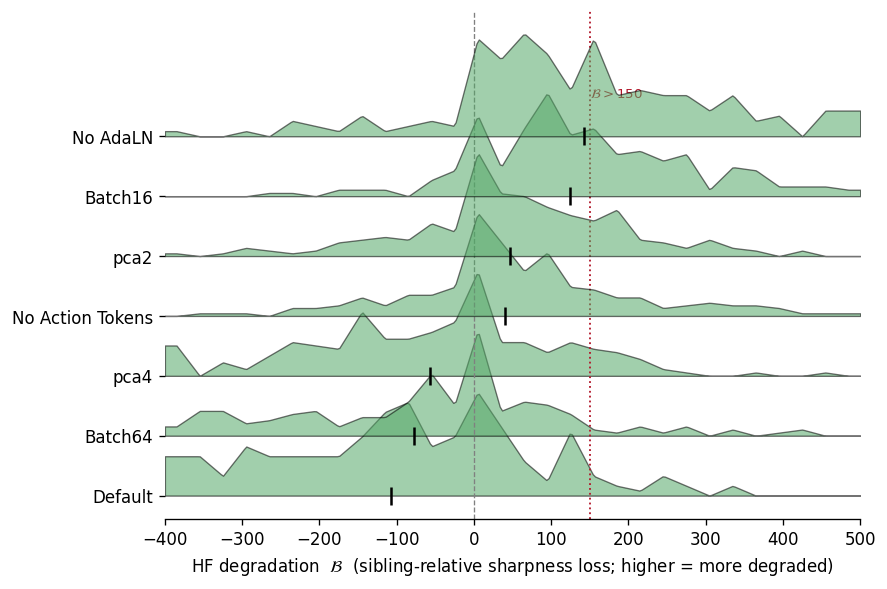
\includegraphics[width=\columnwidth]{Figures/appendix_validation/hf_distribution.png}
    \caption{
        Distribution of the high-frequency-degradation score $\mathcal B$
        (sibling-relative sharpness loss; higher is more degraded). \texttt{No
        AdaLN} and \texttt{Batch16} degrade most, while \texttt{Default},
        \texttt{Batch64}, and \texttt{pca4} lie at or below zero and preserve detail
        better than their same-scene siblings.
    }
    \label{fig:hf_distribution}
\end{figure}

Figure~\ref{fig:hf_fleet_distribution} extends this comparison to the eight
models reported in the main cross-model evaluation, using the same score
definition and evaluation mask. It places the descriptive threshold in context and shows
that the high-frequency failure profiles differ substantially across both our
variants and the external baselines.

\begin{figure}[t]
    \centering
    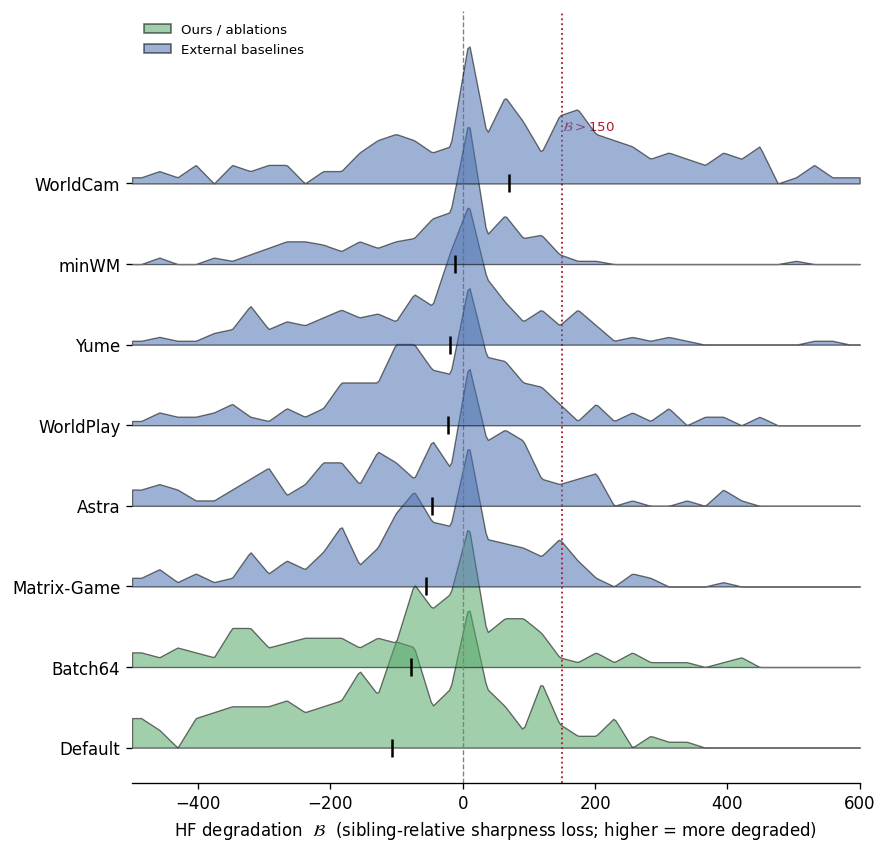
\includegraphics[width=\columnwidth]
    {Figures/appendix_validation/hf_fleet_distribution.png}
    \caption{
        Cross-model distribution of the high-frequency-degradation score
        $\mathcal B$ for the eight models reported in the main comparison, using
        their active evaluation populations ($1{,}809$ rollouts in total). Higher
        values indicate greater sibling-relative loss of sharpness. Green denotes
        our models, while blue denotes external baselines. Black ticks mark
        medians, the grey dashed line marks $\mathcal B=0$, and the red dotted line
        marks the descriptive threshold $\mathcal B>150$.
    }
    \label{fig:hf_fleet_distribution}
\end{figure}

Taken together, the results reveal distinct quality failure modes. Reduced PCA
supervision primarily harms geometric integrity, smaller training batches
increase relocation and progressive loss of detail, and removing the AdaLN
pathway produces weak, drifting continuations with severe high-frequency
degradation. The full-fleet comparison further shows that this degradation is
model-specific rather than an inevitable consequence of long rollouts, with
WorldCam exhibiting the clearest external failure. No single metric therefore
captures overall world-model robustness.


\section{Full Stationary Evaluation}
\label{app:stationary_results}

We give the full stationary evaluation here, we report and analyse both controllability and quality.

Reference-based methods can reward the degenerate strategy of repeating the
final context frame, because this produces little apparent motion even though
the world has frozen. We therefore evaluate the same $32$ contexts using two
complementary quantities: camera stationarity and residual independent scene
animation. A successful null command should hold the viewpoint without
suppressing pedestrians, vehicles, vegetation, or other scene dynamics.

\subsection{Controllability}
\label{app:stationary_controllability}

We apply a stationary command to every model using the protocol in
Appendix~\ref{app:baseline_controls}. For our model, physical zero motion is
obtained by passing an all-zero displacement field through the PCA encoder,
giving the calibrated null action
$a_{\mathrm{null}}=(-0.0234,-0.0013)$. For the external models, we use identity
pose sequences for minWM, WorldPlay, Astra, and WorldCam; an all-zero
keyboard--mouse stream for Matrix-Game; and an explicitly stationary caption
for Yume. These inputs are representable by the released interfaces, but the
published evaluations do not establish that they are learned stationary fixed
points~\cite{minwm,worldcam,astra,matrixgame2,hyworldplay,yume}.

\paragraph{Stationarity}
As in the main controllability evaluation, we track a fixed grid of points in
each rollout. For the stationary test, we fit the dominant coherent motion with
a RANSAC affine transform and use the median inlier displacement as the camera
drift; this should be near zero for a held viewpoint. Against $0.0$\,px in the
real-footage reference, our default model moves by $2.3$\,px, while the other
functional variants lie between $2.0$ and $2.2$\,px. Matrix-Game and WorldPlay
are similarly low-drift at $2.1$ and $2.3$\,px, while minWM reaches $3.0$\,px.
WorldCam drifts by $6.3$\,px; Astra and Yume drift substantially more, by
$19.8$ and $45.9$\,px respectively. The No AdaLN ablation also drifts strongly
at $32.2$\,px. Motion-bearing prompt language contributes to the drift of Yume
and Astra; neutralising it reduces, but does not eliminate, the failure.
Figure~\ref{fig:stat_cont} shows the resulting motion for each model.

\paragraph{Animation}
Low camera drift alone is not sufficient, since a model can remain stationary
by repeating the final context frame and freezing the world. To measure whether
the scene remains alive, we remove the fitted global camera transform and apply
PCA to the residual point trajectories. The remaining localised coherent motion
corresponds to independent movers such as pedestrians, vehicles, and
vegetation. Against a real-footage reference of $1.1$ movers per rollout, our
default model retains $1.4$. In contrast, Matrix-Game and WorldPlay produce
$0.0$ detected movers and therefore freeze the scene, while minWM nearly
freezes with only $0.2$. Several reduced-capacity variants also suppress
animation. The high residual-motion values of strongly drifting models should
not be interpreted as genuine scene activity, since depth-dependent parallax
can remain after the global transform is removed. Table~\ref{tab:anim} reports
both stationarity and animation. A successful no-op must therefore stop the
camera without stopping the world.
\begin{table}[t]
\centering
{
\small
\begin{tabular}{lcc}
\toprule
Model & Movement & Animation \\
\midrule
REAL (reference)        & $0.0$  & $1.1$  \\
\midrule
Ours (Default)          & $2.3$  & $1.4$  \\
Ours (pca4)             & $2.1$  & $0.0$  \\
Ours (pca2)             & $2.2$  & $0.0$  \\
Ours (Batch64)          & $2.0$  & $0.6$  \\
Ours (Batch16)          & $2.0$  & $0.0$  \\
Ours (No Action Tokens) & $2.1$  & $0.1$  \\
Ours (No AdaLN)         & $32.2$ & $6.2$  \\
\midrule
minWM                   & $3.0$  & $0.2$  \\
Matrix-Game             & $2.1$  & $0.0$  \\
WorldPlay               & $2.3$  & $0.0$  \\
WorldCam                & $6.3$  & $2.8$  \\
Astra                   & $19.8$ & $11.2$ \\
Yume                    & $45.9$ & $0.8$  \\
\bottomrule
\end{tabular}
}
\caption{
    Stationarity and animation under a null egomotion command, measured from
    CoTracker tracks over the $32$ stationary contexts. \emph{Movement} is the
    median camera drift in pixels; lower is better. \emph{Animation} is the mean
    number of localised coherent movers after the camera transform is removed.
    A faithful model should remain near the real-footage reference rather than
    freeze to zero. Animation is partly confounded by camera drift through
    residual parallax, so it is interpretable only for low-movement models.
}
\label{tab:anim}
\end{table}

\begin{figure*}[t]
    \centering
    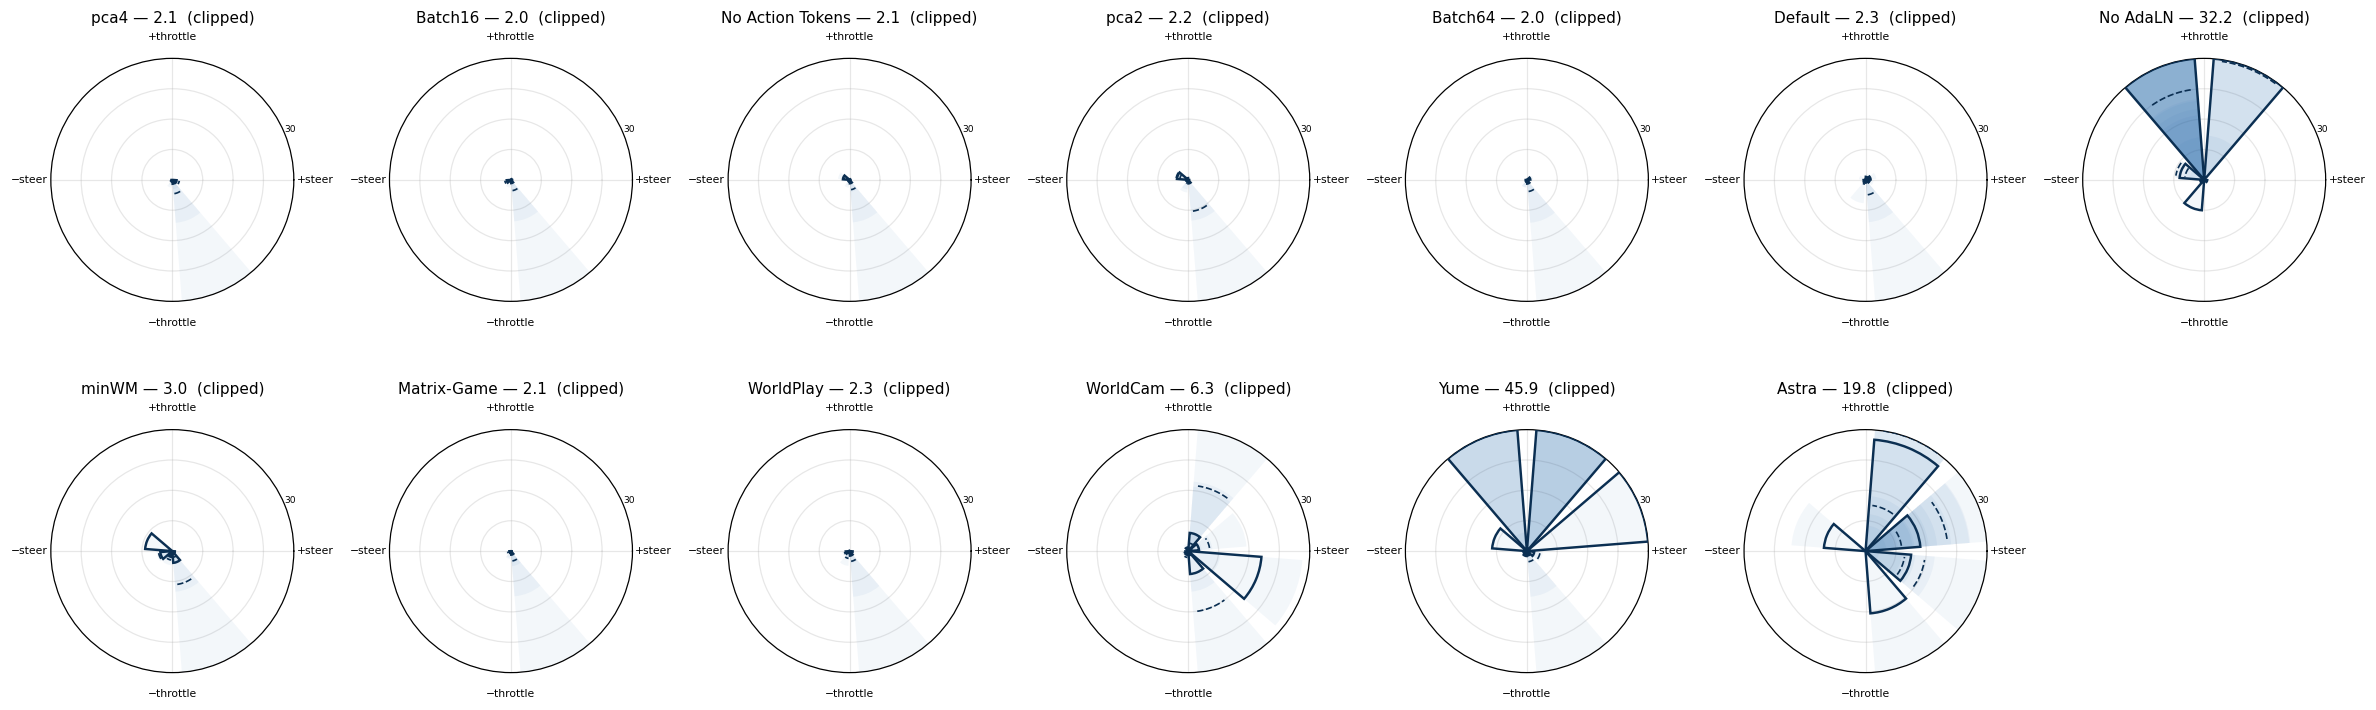
\includegraphics[width=\textwidth]{Figures/stationary_wedges.png}
    \caption{
        Residual egomotion under the null command. Each translucent wedge represents
        one of the $32$ stationary contexts; angle gives the realised drift
        direction and radius its magnitude. Blue denotes forward drift and red
        backward drift. Solid outlines show medians and dashed arcs show
        interquartile ranges.
    }
    \label{fig:stat_cont}
\end{figure*}


\subsection{Quality}
\label{app:stationary_quality}

We apply the five reference-free instruments (style shift, geometric
corruption, scene relocation, conjuring, and high-frequency degradation) to the stationary
(null-command) rollouts. Under a null action a faithful model should be stationary (without scene degradation) but ensure the scene remains animated. These rates measure the scene degradation but we also include a measure of the residual CoTracker outputs when PCA has been applied, as a measure of the animation present in the scene. A completely stationary scene shows that the model only animates scenes while it moves, indicative of a low agent---world separation.
Table~\ref{tab:stationary_quality} reports the results.

Our full-capacity variants are essentially inert in the correct sense: they hold
$0\%$ style shift and $0\%$ geometric corruption and relocate in only $3\%$ of
rollouts, i.e.\ they keep the scene still and intact when told to do nothing. The
external baselines do not. Matrix-Game corrupts geometry in $94\%$ of stationary
rollouts and Astra in $44\%$ (with $31\%$ relocation), so a null command sends
them into malformed or entirely different scenes rather than a held pose.
Relocation is the most common external failure---Astra $31\%$, Yume $19\%$,
WorldCam $16\%$---confirming that these models cannot simply stay in place.

The one ablation that stands out is \texttt{noadaln}, which washes out in $66\%$
of stationary rollouts (median $\mathcal B=+282$) and relocates in $9\%$. This
matches its behaviour elsewhere: with the AdaLN action pathway removed it
produces weak, drifting continuations even when the command asks for none. The
smaller \texttt{Batch16} and lower-dimension \texttt{pca2} variants show mild
high-frequency degradation ($12\%$ and $9\%$) but otherwise remain stable.
